\documentclass[12pt,a5paper]{article}

% English language
\usepackage[utf8]{inputenc}
\usepackage[T1]{fontenc}

% Page layout
\usepackage[a5paper,margin=1.5cm]{geometry}
\usepackage{setspace}
\setstretch{1.06}

% Graphics and figures
\usepackage{graphicx}
\usepackage{float}

% Tables
\usepackage{longtable}
\usepackage{booktabs}
\usepackage{array}
\usepackage{tabularx}

% Mathematics
\usepackage{amsmath}
\usepackage{amssymb}
\usepackage{amsthm}
\newcommand{\Kcal}{\mathcal{K}}

% Hyperlinks
\usepackage{hyperref}
\hypersetup{
    colorlinks=true,
    linkcolor=black,
    citecolor=black,
    urlcolor=black
}

% Headers and footers
\usepackage{fancyhdr}
\pagestyle{fancy}
\fancyhf{}
\renewcommand{\headrulewidth}{0pt}
\fancyfoot[C]{\thepage}

% Section formatting
\usepackage{titlesec}
\titleformat{\section}{\centering\normalsize\bfseries}{\thesection}{1em}{}
\titleformat{\subsection}{\normalsize\bfseries}{\thesubsection}{1em}{}

% Reduce spacing
\titlespacing*{\section}{0pt}{8pt}{4pt}
\titlespacing*{\subsection}{0pt}{6pt}{3pt}

% Paragraph settings
\setlength{\parindent}{1.25cm}
\setlength{\parskip}{0pt}

\begin{document}
\sloppy

% Suppress page number on first page
\thispagestyle{empty}

% ============================================================
% TITLE PAGE
% ============================================================
\begin{center}
\textbf{National Research Nuclear University MEPhI}

\vspace{1cm}

\textit{As a manuscript}

\vspace{2cm}

\textbf{Roger Nick Anaedevha}

\vspace{1.5cm}

{\large \textbf{Development of Adversarial Resilient Models
Based on Artificial Intelligence in Hybrid Intrusion
Detection and Prevention Systems for Network Security}}

\vspace{1.5cm}

\textbf{2.3.1.\ Systems Analysis, Information Management\\
and Processing, Statistics\\
(Technical Sciences)}

\vspace{2cm}

\textbf{ABSTRACT}

\vspace{0.5cm}

of a dissertation for the degree of\\
Candidate of Technical Sciences

\vfill

Moscow -- 2026
\end{center}

\newpage

% ============================================================
% PAGE 2 — Committee and defence details
% ============================================================
\thispagestyle{empty}
\enlargethispage{1cm}

{\footnotesize
\begin{center}
\textbf{The work was carried out at the Federal State Autonomous\\
Educational Institution of Higher Education\\
``National Research Nuclear University MEPhI''}
\end{center}

\vspace{0.2cm}

\noindent\begin{tabular}{@{}p{3cm}p{7.2cm}@{}}
\textbf{Scientific supervisor:} & \textbf{Trofimov Alexander Gennadievich} \newline Doctor of Physical and Mathematical Sciences, Professor, Professor of Dept.\ No.~22 ``Cybernetics'' of NRNU MEPhI \\
\end{tabular}

\vspace{0.2cm}

\noindent\textbf{Official opponents:}
\vspace{0.05cm}

\noindent\begin{tabular}{@{}p{3cm}p{7.2cm}@{}}
Doctor of Technical Sciences, Professor, Laureate of the Presidential Prize of the RF in Education, Honorary Worker of Science and High Technology of the RF \newline \textbf{Eremeev Alexander Pavlovich} &
Professor of the Department of Applied Mathematics and Artificial Intelligence of the National Research University MEI \\[0.15cm]

Doctor of Technical Sciences, Professor \newline \textbf{Kalyanov Georgy Nikolaevich} &
Chief Researcher of the Laboratory of Infrastructure Systems, V.A.~Trapeznikov Institute of Control Sciences of the Russian Academy of Sciences \\
\end{tabular}

\vspace{0.2cm}

\noindent\begin{tabular}{@{}p{3cm}p{7.2cm}@{}}
\textbf{Leading organisation:} & Federal State Budgetary Educational Institution of Higher Education ``Tver State Technical University'' \\
\end{tabular}

\vspace{0.2cm}

\noindent The defence will take place on 30.06.2026 at a meeting of the Dissertation Council~2.01 of FGAOU VO ``NRNU MEPhI'' (115409, Moscow, Kashirskoe shosse, 31)

\vspace{0.15cm}

\noindent The dissertation is available in the library and on the website \url{https://ds.mephi.ru/} of FGAOU VO ``NRNU MEPhI''

\vspace{0.15cm}

\noindent The abstract was distributed \underline{\hspace{2.5cm}} 2026

\vspace{0.3cm}

\noindent\begin{tabular}{@{}p{4.5cm}p{2cm}p{3.5cm}@{}}
Scientific Secretary of the Dissertation Council, Candidate of Physical and Mathematical Sciences & & Klimanov Sergey Gennadievich \\
\end{tabular}
}

\newpage

% ============================================================
% MAIN CONTENT BEGINS
% ============================================================
\setcounter{page}{3}

\section*{GENERAL CHARACTERISTICS OF THE WORK}
\addcontentsline{toc}{section}{General Characteristics of the Work}

\subsection*{Relevance of the research topic and the degree of its development}

Hybrid Intrusion Detection and Prevention Systems (Hybrid~IDPS)
constitute the principal defensive contour of mission-critical
information and telecommunication systems~--- network-traffic
backbones, hardened data-centre segments, unmanned-aerial-vehicle
infrastructures, banking and financial platforms, medical
information systems, the industrial Internet of Things, and
the control of critical infrastructures. In contrast to
conventional commercial products (Snort, Suricata, Zeek,
Cisco~IPS, Palo~Alto, McAfee), which rely exclusively on
signature analysis and fixed rule sets, the present work
defines Hybrid~IDPS as an \emph{AI/ML-augmented} defensive
contour that combines the three canonical detection types~---
signature-based, behavioural (anomaly-based), and
protocol-analysis-based~--- into a single multi-tier
architecture with learnable components and integrated response
facilities.

Incident analyses over the past five years in healthcare,
finance, industrial IoT, autonomous systems, and cybersecurity
itself show that the robustness of deployed Hybrid~IDPS lags
their detection accuracy by 25--65~percentage points: systems
that demonstrate 95--98\% accuracy on benchmark data lose
20--40\% under adversarial perturbations of inputs, drift of
traffic distributions, Byzantine participants in distributed
training, and protocol-profile evolution. The fundamental
inefficiencies of modern Hybrid~IDPS include: a signature lag
of 30--90~days behind newly emerging threats, a false-alert rate
of $10^{-2}$--$10^{-1}$ per normal flow, and the quadratic
$\mathcal{O}(P\cdot S)$ cost of real-time protocol analysis in
the number of protocols and sessions. Accordingly, the present
work is devoted to the \emph{development of adversarial
resilient models based on artificial intelligence in hybrid
intrusion detection and prevention systems for network
security}, with the distributed and non-stationary properties
(P4, P6) retained in full as mandatory requirements on the
developed AI-based models within the invariant P1--P6 matrix.

In this dissertation, a unified formalisation of Hybrid~IDPS is
introduced as the tuple $\mathcal{H} = (\mathcal{V}_t,
\mathcal{E}_t, X_t, A_t, f_\theta, g_\psi, \pi)$, where
$\mathcal{V}_t$ and $\mathcal{E}_t$ denote the time-varying
entity and connection sets, $X_t$ is the feature matrix,
$A_t$ collects the active signatures and rules, $f_\theta$ is
the learnable detection module, $g_\psi$ the confidence
module, and $\pi$ the response policy. Six cross-cutting
properties of Hybrid~IDPS~--- adversarial resilience~(P1),
robustness~(P2), efficiency~(P3), distributed environment~(P4),
the human factor~(P5), and non-stationarity~(P6)~--- are
formalised as invariant conditions and systematically
decomposed into seven sub-problems addressed by seven novel
Models and algorithms~M1--M7. Graph neural networks are
employed in this work as one branch of the family of
learnable models applicable to Hybrid~IDPS, alongside
statistical, classical~ML, hybrid, and game-theoretic
approaches.

Substantial contributions to the disciplines forming the
methodological foundation of the work have been made by
researchers including: in intrusion detection and prevention
and network security~--- A.\,A.~Burlakov, A.\,S.~Markov,
V.\,V.~Sachkov, M.~Roesch, V.~Paxson; in graph deep
learning~--- T.\,N.~Kipf, M.~Welling, P.~Veli\v{c}kovi\'{c},
W.\,L.~Hamilton; in neural ODEs and state-space models~---
R.\,T.\,Q.~Chen, A.~Gu, T.~Dao; in adversarial machine
learning~--- A.~Madry, N.~Carlini, D.~Wagner; in federated
learning with privacy~--- B.~McMahan, K.~Bonawitz,
H.~B.~McMahan; and in game theory and robustness
certification~--- A.~Sinha, J.~Steinhardt, J.~Cohen. However,
no existing approach jointly satisfies the four requirements~---
robustness, accuracy, efficiency, and privacy~--- across all
three operating conditions of Hybrid~IDPS: adversarial
environments, non-stationarity, and distributed training
dynamics. This contradiction between multi-dimensional
requirements and the current state of the algorithmic base
determines the relevance of the present research.

\subsection*{Object and subject of research}

\textbf{The object of research} is \emph{Hybrid Intrusion
Detection and Prevention Systems} (Hybrid~IDPS) operating in
adversarial, non-stationary, and distributed environments and
adaptable to a variety of application domains~---
network-traffic protection, UAV systems, banking and financial
infrastructure, medical-data storage, the industrial Internet
of Things, and the control of critical infrastructures. A
Hybrid~IDPS combines signature-based, behavioural,
protocol-analysis, and learning-based components into a single
defensive contour with a multi-tier architecture and integrated
response facilities.

\textbf{The subject of research} comprises the models,
algorithms, and special mathematical support that improve the
robustness and efficiency of Hybrid~IDPS while preserving
adversarial resilience, the privacy of distributed data, and
the calibration of uncertainty estimates~--- including the
apparatus of continuous-time graph dynamics, selective
state-space models, federated optimisation with differential
privacy, optimal transport, Bayesian inference, and
game-theoretic certification.

\subsection*{Research objective and tasks}

\textbf{The objective} of this dissertation is to improve the
robustness and efficiency of Hybrid Intrusion Detection and
Prevention Systems (Hybrid~IDPS) operating under adversarial,
non-stationary, and distributed conditions, by developing a
unified mathematical description of Hybrid~IDPS together with
a consistent family of Models and algorithms~M1--M7, and to
demonstrate the applicability of the results by instantiating
the framework in the network-traffic protection sector (NIDPS)
and transferring it to the adjacent sector of onboard
unmanned-aerial-vehicle systems.

\textbf{Tasks:}

\begin{enumerate}
\item Systematise existing approaches to building Hybrid~IDPS
across seven application sectors, identify the open gaps, and
formulate uniform requirements for the developed models and
algorithms.

\item Construct a unified mathematical description of
Hybrid~IDPS as the tuple
$\mathcal{H} = (\mathcal{V}_t, \mathcal{E}_t, X_t, A_t,
f_\theta, g_\psi, \pi)$ and formalise the six cross-cutting
properties P1--P6 as invariant conditions, organising them as a
$3\times4$ condition--requirement matrix.

\item Develop seven Models and algorithms~M1--M7 that jointly
cover all twelve cells of this matrix: continuous-time graph
dynamics CT-TGNN/SDE-TGNN~(M1); federated optimisation
FedLLM-API with differential privacy~(M2); multi-level
temporal embeddings TripleE-TGNN~(M3); selective state-space
model MambaShield~(M4); uncertainty-calibrated inference
Stochastic Transformer/UC-HGP~(M5--M6); and game-theoretic
certification FedGTD~(M7).

\item Instantiate Hybrid~IDPS in the NIDPS sector by developing
a formal data-to-graph transformation pipeline, a unified
34-class attack taxonomy, and an 83-feature engineering
pipeline consistent with the models M1--M7.

\item Conduct experimental validation of the developed models
and algorithms on six benchmark datasets totalling over
84.2~million labelled samples and 84~unique attack categories,
using a unified 23-metric framework spanning accuracy,
calibration, uncertainty, adversarial robustness, computational
efficiency, and privacy.

\item Implement a production-grade software platform
\textbf{RobustIDPS.ai} that integrates 17~neural-network models
into 10~functional groups and 51~pages of a Progressive Web
Application, and obtain industrial validation through
implementation acts from three organisations.

\item Confirm the domain independence of the developed
framework by transferring it to the adjacent sector of UAV
onboard systems with a three-tier
``onboard~-- droneport~-- cloud'' architecture, and by
experimentally demonstrating cross-domain transfer to speech
processing and medical time series.
\end{enumerate}

\subsection*{Methodology and methods of research}

The work employed methods of systems analysis, graph theory
and spectral graph theory, ordinary and stochastic differential
equations, functional analysis, optimal transport theory,
deep learning, Bayesian inference, information theory, game
theory (Stackelberg and Nash equilibria), optimisation theory,
probability theory, mathematical statistics, the theory of
differential privacy, and numerical and computational
experiments on benchmark corpora. The methodology provides a
unified formal description of Hybrid~IDPS at the level of the
tuple model and the six invariant properties, which lets the
mathematical results M1--M7 be rigorously linked to the applied
goal of improving robustness and efficiency.

\subsection*{Scientific novelty of the work}

\begin{enumerate}
\item \textit{Unified mathematical description of Hybrid~IDPS.}
For the first time, a tuple formalisation of Hybrid~IDPS
$\mathcal{H} = (\mathcal{V}_t, \mathcal{E}_t, X_t, A_t,
f_\theta, g_\psi, \pi)$ is proposed, together with a
companion system of six invariant properties P1--P6 covering
adversarial resilience, robustness, efficiency, distributed
environment, the human factor, and non-stationarity. On this
basis, a $3\times4$ condition--requirement matrix is
constructed, organising the M1--M7 family as a covering of all
twelve cells.

\item \textit{Continuous-time temporal graph dynamics for
Hybrid~IDPS (CT-TGNN, SDE-TGNN).} For the first time within a
Hybrid~IDPS, a model is used in which node representations
evolve under neural ordinary differential equations on
time-varying graphs, and certified robustness bounds are
derived from the Gr\"{o}nwall inequality. The stochastic
extension SDE-TGNN replaces deterministic dynamics with It\^{o}
equations and analytically propagates the first two moments
through the Fokker--Planck equation. Achieved: F1 99.0\%, ECE
0.042, certified robustness 76.2\% at perturbation radius
$R{=}0.25$, and cross-domain transfer of 90.5\% F1 without
fine-tuning.

\item \textit{Byzantine-resilient federated optimisation for
Hybrid~IDPS (FedLLM-API).} An original federated optimiser has
been developed that jointly provides coordinate-wise
trimmed-mean aggregation, $(\varepsilon{=}0.85,\,\delta{=}10^{-5})$
differential privacy, and Wasserstein-distance distributional
alignment for heterogeneous clients. Convergence at
$\mathcal{O}(1/\sqrt{T})$ is proved under 30\% corrupted
participants; with 40\% Byzantine participants, the system
achieves 87.1\% accuracy against 61.4\% for FedAvg. LLM
integration enables 87.6\% F1 on zero-shot detection of novel
attack classes.

\item \textit{Multi-level temporal graph embeddings for
Hybrid~IDPS (TripleE-TGNN).} A triple-embedding architecture
at service, trace, and node levels with dual
temporal--spatial attention and elastic weight consolidation
against catastrophic forgetting has been developed. Achieved
accuracy of 96.8\% with 40\% reduction in computational cost
and 94.7\% accuracy maintained without retraining under
continuous topology evolution.

\item \textit{Selective state-space models for Hybrid~IDPS
(MambaShield).} An architecture has been developed that uses
FFT convolutions to reduce inference complexity from
$\mathcal{O}(L^{2})$ to $\mathcal{O}(L\log L)$, and integrates
progressive adversarial robustness distillation. Under 25\%
training-time poisoning, the model achieves 91.4\% accuracy
versus 73.8\% for undefended training; PAC-Bayesian
generalisation certificates confirm the bound with 2.7\%
margin; inference latency is 0.5~ms per flow.

\item \textit{Uncertainty-calibrated inference for Hybrid~IDPS
(Stochastic Transformer, UC-HGP).} For the first time within
a Hybrid~IDPS, variational Bayesian attention has been
integrated with hierarchical Gaussian processes to provide
epistemic--aleatoric uncertainty decomposition with ECE of
0.078 (a 59\% reduction over deterministic attention) and a
43\% reduction in analyst workload through uncertainty-driven
triage.

\item \textit{Game-theoretic certification of Hybrid~IDPS
(FedGTD).} An original robustness-certification mechanism has
been constructed via Stackelberg equilibria with a
multiplicative-weights algorithm for which the regret bound
$R(T)\le 2\sqrt{T\log|\mathcal{C}|}$ is proved. A consistency
regulariser couples all seven models with proven convergence.
Accuracy of 94.7\% against adaptive adversaries versus 87.6\%
for non-strategic approaches.

\item \textit{Domain-specific foundation model (CyberSecLLM).}
A novel architecture with ODE-augmented selective state-space
blocks has been developed, achieving 89.1\% average zero-shot
accuracy on the 11-task CyberSecBench evaluation~--- a
20.5-point improvement over GPT-4~--- while processing
million-token graph event sequences in 2.3~seconds.
\end{enumerate}

\subsection*{Theoretical significance}

The theoretical significance lies in the construction of a
unified mathematical description of Hybrid~IDPS as the object
of investigation and of an integrated system of proofs that
connects five formal disciplines: neural ordinary and
stochastic differential equations (CT-/SDE-TGNN, MambaShield);
optimal transport and the theory of differential privacy
(FedLLM-API); selective state-space models and FFT
convolutions (MambaShield); variational Bayesian inference
and hierarchical Gaussian processes (Stochastic Transformer,
UC-HGP); and game theory with stochastic no-regret learning
(FedGTD). Joint use of these tools yields formal guarantees of
convergence, stability, privacy, and generalisation that are
verified both theoretically and empirically, and unifies these
disciplines into a single scientific--methodological framework
for improving the robustness and efficiency of Hybrid~IDPS.

\subsection*{Practical significance}

The practical significance is determined by the development of
models, algorithms, and special software for constructing
Hybrid~IDPS applicable in the network-traffic protection
sector, UAV onboard systems, banking and financial
infrastructure, medical information systems, the industrial
Internet of Things, and other domains. The developed system
provides:

\begin{itemize}
\item high detection accuracy (94.7\% on CIC-IoT-2023) with
simultaneous adversarial resilience;
\item preservation of data privacy in distributed architectures
through federated learning with
$(\varepsilon{=}0.85,\,\delta{=}10^{-5})$ differential privacy;
\item real-time operation: 8.7~million events/second at 47~ms
latency, with 0.5~ms/flow inference for MambaShield;
\item forward compatibility with evolving protocols, including
post-quantum cryptographic standards (Multi-Agent~PQC-IDS
module, 96.2\% accuracy);
\item cross-domain portability: 90.5\% F1 without fine-tuning,
confirmed on speech (LibriSpeech) and medical (MIMIC-III/eICU)
corpora.
\end{itemize}

Practical significance is confirmed by the release of the
software platform \textbf{RobustIDPS.ai}
(DOI:~10.5281/zenodo.19129512), which integrates
\textbf{17~neural-network models} into \textbf{10~functional
groups} and \textbf{51~pages} of a Progressive Web Application,
a four-layer LLM defence framework (94.5\% detection across
517 attack scenarios with four commercial backends), and a
Multi-Agent~PQC-IDS module; the platform is corroborated by
two received implementation acts: from NII~IKT~LLC (Novosibirsk;
integration of poisoning-resilient anomaly-detection models into
the operating intrusion-detection system of the organisation and
active use of the RobustIDPS.ai platform by in-house cybersecurity
specialists) and from Ksyrix~LLC (Moscow; deployment of the
developed solutions within the company's network-traffic
analysis and infrastructure-protection system for multi-stage
attack detection, uncertainty-based identification of previously
unknown patterns, and adaptation to changes in traffic
statistics); the act from the Artificial Intelligence Center of
NRNU~MEPhI, Moscow (deployment to UAV onboard systems), is in
the course of formalisation.

\subsection*{Reliability of scientific results}

Reliability is ensured by: a strict mathematical formalisation
of Hybrid~IDPS as a tuple model and six properties P1--P6 with
proofs of convergence, stability, privacy, and complexity;
experimental validation on six open datasets totalling
84.2~million labelled samples and 84~unique attack categories;
comparative analysis with modern baselines and state-of-the-art
methods, demonstrating superiority by 2.9--5.6~percentage
points; ablation studies confirming the measurable contribution
of each component M1--M7; experiments under six families of
adversarial attacks; cross-domain transfer; presentation at
international conferences; publications in leading peer-reviewed
journals (Scopus/Web of Science); and implementation acts from
three organisations.

\subsection*{Validation of research results}

The main provisions and results were presented and discussed at
the following international and Russian scientific conferences:

\begin{enumerate}
\item 2024 Conference of Young Researchers in Electrical and Electronic Engineering (ElCon-2024), Saint Petersburg, Russia, IEEE;
\item 2025 Conference of Young Researchers in Electrical and Electronic Engineering (ElCon-2025), ETU-LETI, Saint Petersburg, Russia, IEEE;
\item International Conference ``Advances in Neural Computation, Machine Learning, and Cognitive Research IX'' (NEUROINFORMATICS-2025), Springer;
\item Third All-Russian Scientific and Technical Conference ``Cybernetics and Information Security'' (KIB-2025), NRNU MEPhI, Moscow;
\item 2026 IEEE 27th International Conference of Young Professionals in Electron Devices and Materials (EDM-2026), Altai Republic, Russia;
\item 11th IEEE Electronics System-Integration Technology Conference (IEEE ESTC 2026), Helsinki, Finland;
\item IEEE Research and Technologies for Society and Industry (RTSI) 2026 Conference, Espoo, Finland;
\item NeurIPS 2026: The 40th Annual Conference on Neural Information Processing Systems, Sydney, Australia.
\end{enumerate}

\subsection*{Publications}

The main results have been published in 18 scientific works,
including: 5~articles in peer-reviewed journals indexed in
Scopus and Web of Science (Neurocomputing, Expert Systems with
Applications, Complex and Intelligent Systems, Optical Memory
and Neural Networks, IJASRE); 4~papers in proceedings of
international conferences (Scopus, IEEE~Xplore); 2~articles
accepted for publication (Knowledge and Information Systems,
Complex and Intelligent Systems); 7~articles under review at
leading IEEE~Transactions journals and other venues.

\subsection*{Main scientific results submitted for defence}

The results submitted for defence are listed in the order
reflecting their logical dependencies within the unified
mathematical description of Hybrid~IDPS; each subsequent result
builds on the guarantees established by its predecessors.

\begin{enumerate}
\item A unified mathematical description of Hybrid~IDPS as
the tuple $\mathcal{H} = (\mathcal{V}_t, \mathcal{E}_t, X_t,
A_t, f_\theta, g_\psi, \pi)$ and a system of six invariant
properties P1--P6 that form a $3\times4$ condition--requirement
matrix, on the basis of which the M1--M7 family is constructed.

\item Models CT-TGNN and SDE-TGNN of certified continuous-time
graph dynamics, in which neural ODEs/SDEs govern node and edge
evolution on time-varying topologies, and certified robustness
bounds are derived from the Gr\"{o}nwall inequality and from
analytical moment propagation through the Fokker--Planck
equation.

\item The FedLLM-API algorithm for Byzantine-resilient
federated optimisation, with proven convergence at
$\mathcal{O}(1/\sqrt{T})$, formal differential privacy
$(\varepsilon{=}0.85,\,\delta{=}10^{-5})$, and optimal-transport
distributional alignment, enabling collaborative training of
Hybrid~IDPS participants under Byzantine adversaries and a
controlled privacy budget.

\item The TripleE-TGNN architecture for multi-level temporal
graph embeddings and the MambaShield architecture for selective
state-space inference with complexity $\mathcal{O}(L\log L)$,
which jointly satisfy the efficiency and poisoning-resilience
requirements of Hybrid~IDPS under continuous topology
evolution.

\item Models Stochastic Transformer and UC-HGP for
uncertainty-calibrated inference with epistemic--aleatoric
decomposition and a sub-linear regret bound, supporting
adaptation of Hybrid~IDPS to non-stationary distributions and
human-factor support (analyst triage and prioritisation).

\item The FedGTD game-theoretic certification framework that
integrates the guarantees of results~(2)--(5) into a single
evaluation methodology via Stackelberg equilibria and
consistency regularisation, and the domain-specific foundation
model CyberSecLLM.

\item Software implementation of the results as the
RobustIDPS.ai platform with 17~neural-network models in
10~functional groups and 51~pages of the web application,
validated on six benchmark datasets (84.2~million samples,
84~attack categories) and corroborated by four implementation
acts, together with instantiation of the same framework in the
adjacent sector of UAV onboard systems.
\end{enumerate}

\subsection*{Conformity with the passport of the scientific specialty}

The dissertation corresponds to specialty 2.3.1 ``Systems
Analysis, Information Management and Processing, Statistics'':

\noindent P.4 ``Development of methods and algorithms for
solving problems of system analysis, optimisation, management,
decision-making, information processing and artificial
intelligence.''~--- conformity is confirmed by the development
of seven original Models and algorithms~M1--M7 for the tasks
of intrusion detection and prevention and the processing of
graph traffic streams within Hybrid~IDPS.

\noindent P.5 ``Development of special mathematical and
algorithmic support for systems of analysis, optimisation,
control, decision-making, information processing and
artificial intelligence.''~--- conformity is confirmed by the
formalisation of Hybrid~IDPS as a tuple model and six
invariant properties P1--P6 and by the implementation of the
unified RobustIDPS.ai software platform with 17~integrated
neural-network models.

\subsection*{Structure and scope of the dissertation}

The dissertation consists of an Introduction, six chapters, a
Conclusion, a bibliographic list, and three appendices. The
main text is 230~pages. The bibliography contains 204~entries.
Chapter~1 provides a systems analysis of Hybrid~IDPS in seven
application sectors and identifies the open gaps. Chapter~2
develops the unified mathematical description of Hybrid~IDPS
and the family of Models M1--M7. Chapter~3 instantiates this
description in the NIDPS sector. Chapter~4 presents the
experimental validation. Chapter~5 describes the RobustIDPS.ai
software platform. Chapter~6 demonstrates the transfer of the
developed framework to the sector of UAV onboard systems.

\section*{MAIN CONTENT OF THE WORK}
\addcontentsline{toc}{section}{Main Content of the Work}

\textbf{The Introduction} substantiates the relevance of the
topic, defines the object (Hybrid~IDPS) and subject (models and
algorithms for improving robustness and efficiency), states the
research objective and the seven tasks, sets out the scientific
novelty, the theoretical and practical significance, the main
results submitted for defence, the validation of the work, and
the structure of the dissertation.

\textbf{Chapter~1} provides a systems analysis of Hybrid~IDPS
across seven application sectors (network-traffic protection,
banking and finance, healthcare, industrial IoT, UAV onboard
systems, cloud and microservices environments, and public
administration and critical infrastructure) and records the
gaps that cannot be closed within a single model. The chapter
describes the three canonical detection types (signature,
behavioural, protocol-analysis), identifies their limitations,
and formulates the requirements for the developed models and
algorithms. Figure~\ref{fig:nidps_overview} shows the executive
overview of the NIDPS contour as one of the principal
instantiations of Hybrid~IDPS.

% ============================================================
% FIGURE 1: NIDPS Executive Overview
% ============================================================
\begin{figure}[H]
\centering
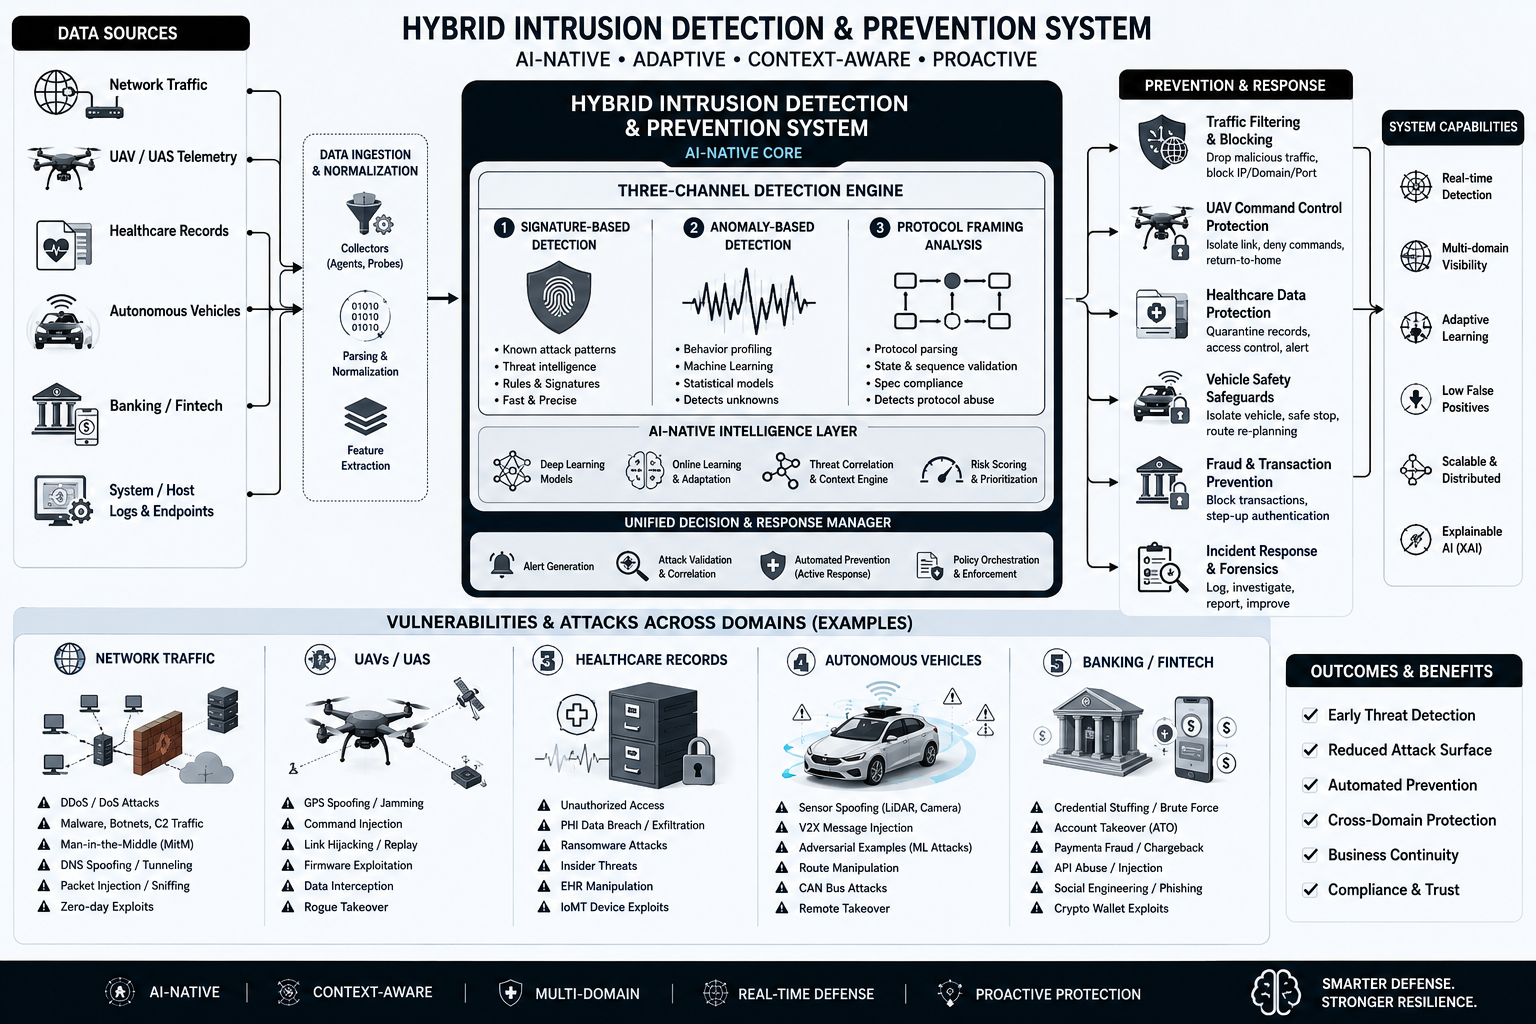
\includegraphics[width=0.92\textwidth]{figures/fig_nidps_v1.png}
\caption{Executive overview of the network instantiation of
Hybrid~IDPS (NIDPS): a learnable contour atop signature and
behavioural detectors}
\label{fig:nidps_overview}
\end{figure}

\textbf{Chapter~2} formalises Hybrid~IDPS as the tuple
$\mathcal{H} = (\mathcal{V}_t, \mathcal{E}_t, X_t, A_t,
f_\theta, g_\psi, \pi)$ and the six invariant properties
P1--P6 (Figure~\ref{fig:main_arch}). On this basis, the M1--M7
family is constructed as a covering of the $3\times4$
condition--requirement matrix.

% ============================================================
% FIGURE 2: Research Framework Matrix
% ============================================================
\begin{figure}[H]
\centering
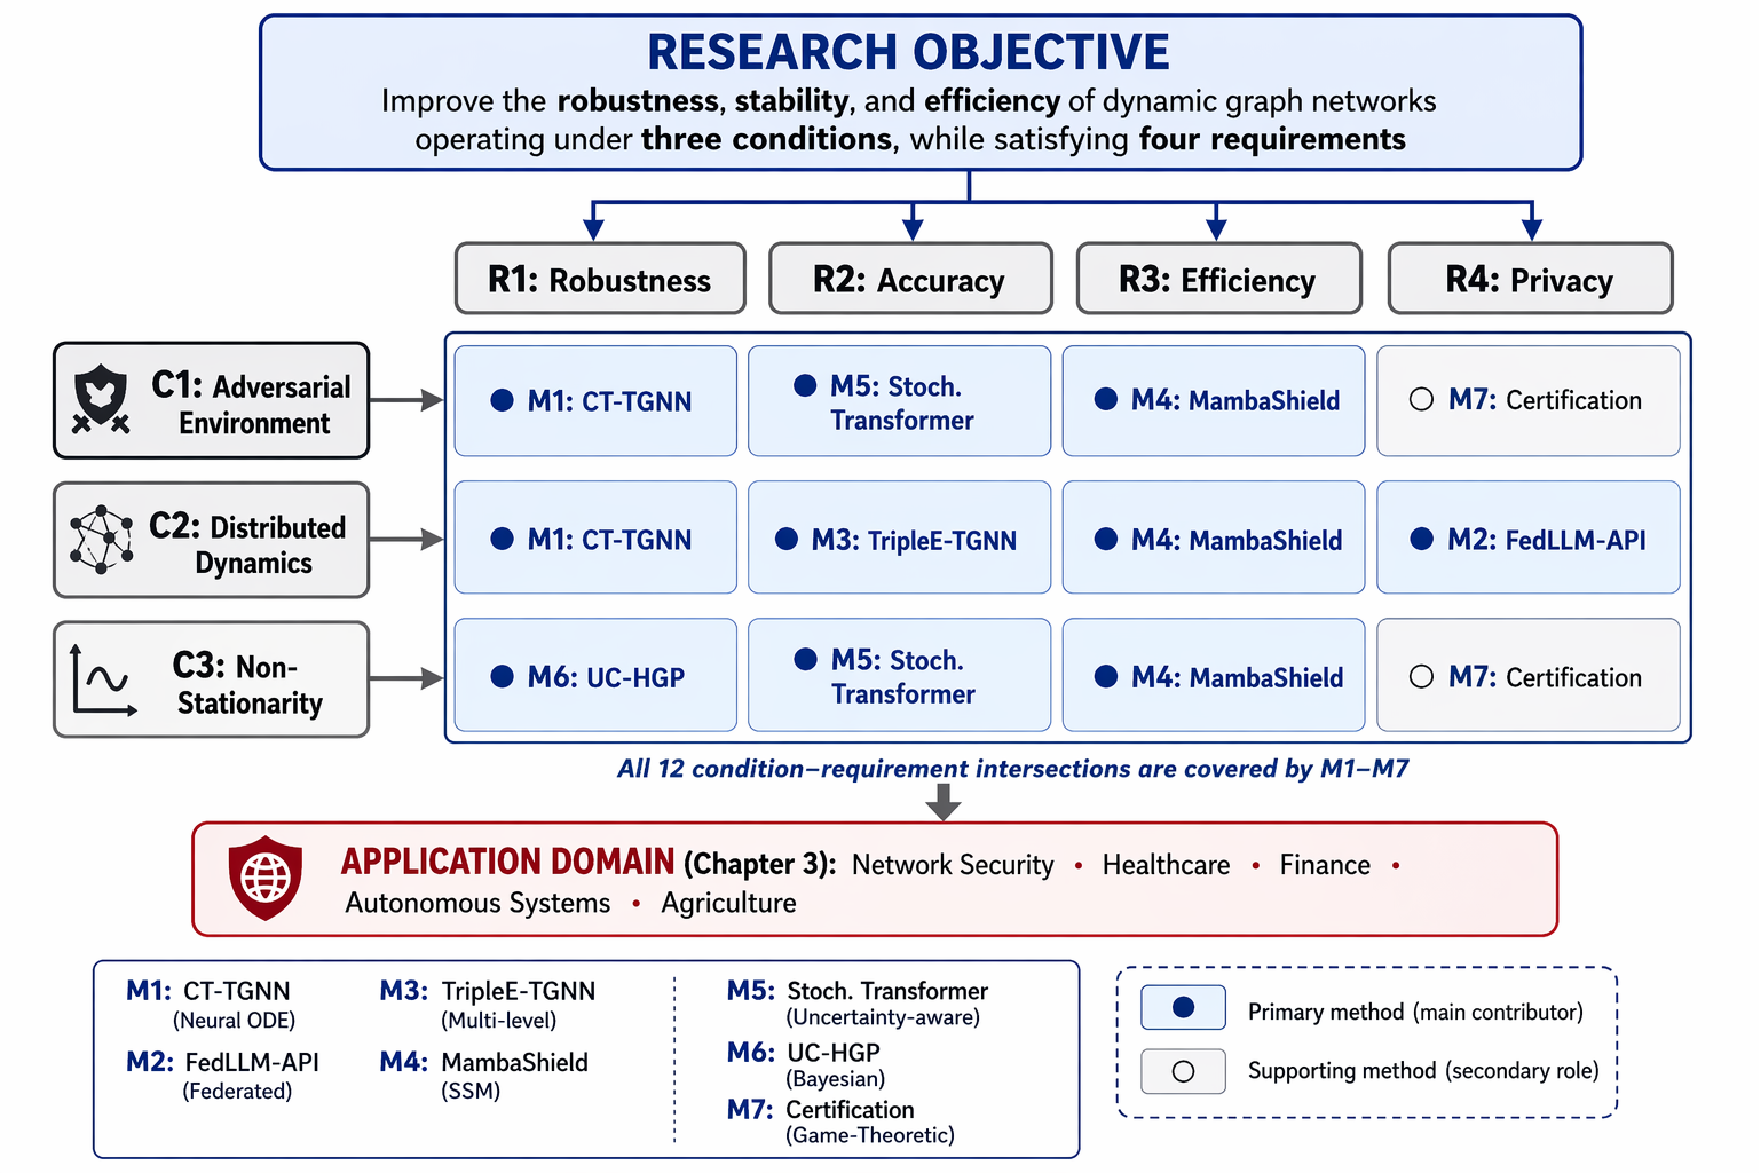
\includegraphics[width=0.96\textwidth]{figures/Main_arch_v1.pdf}
\vspace{-0.5cm}
\caption{Architectural foundation of the unified mathematical
description of Hybrid~IDPS: the M1--M7 family covers all
twelve cells of the condition--requirement matrix}
\label{fig:main_arch}
\end{figure}

\textit{Model M1: CT-TGNN/SDE-TGNN --- continuous-time graph
dynamics for Hybrid~IDPS.} The evolution of node representations
is governed by a parameterised differential operator on a
time-varying topology:
\begin{equation}
\frac{dh_v(t)}{dt} = f_\theta\bigl(h_v(t), A(t), X(t), t\bigr).
\end{equation}
The adjoint sensitivity method provides $\mathcal{O}(1)$ memory
training; temporal adaptive batch normalisation reconciles the
continuous dynamics with normalisation layers.

\textbf{Theorem~1 (Convergence).} For Lipschitz constant $L_f$
and learning rate $\eta < 2/L_f$, training converges at rate
$\mathcal{O}(1/\sqrt{T})$.

\textbf{Theorem~2 (Certified robustness).} For input
perturbations $\|\delta X\|\le\varepsilon$, the output
sensitivity is bounded via the Gr\"{o}nwall inequality by
$\|\delta h(T)\|\le\varepsilon L_g T\exp(L_g T)$.

\begin{figure}[H]
\centering
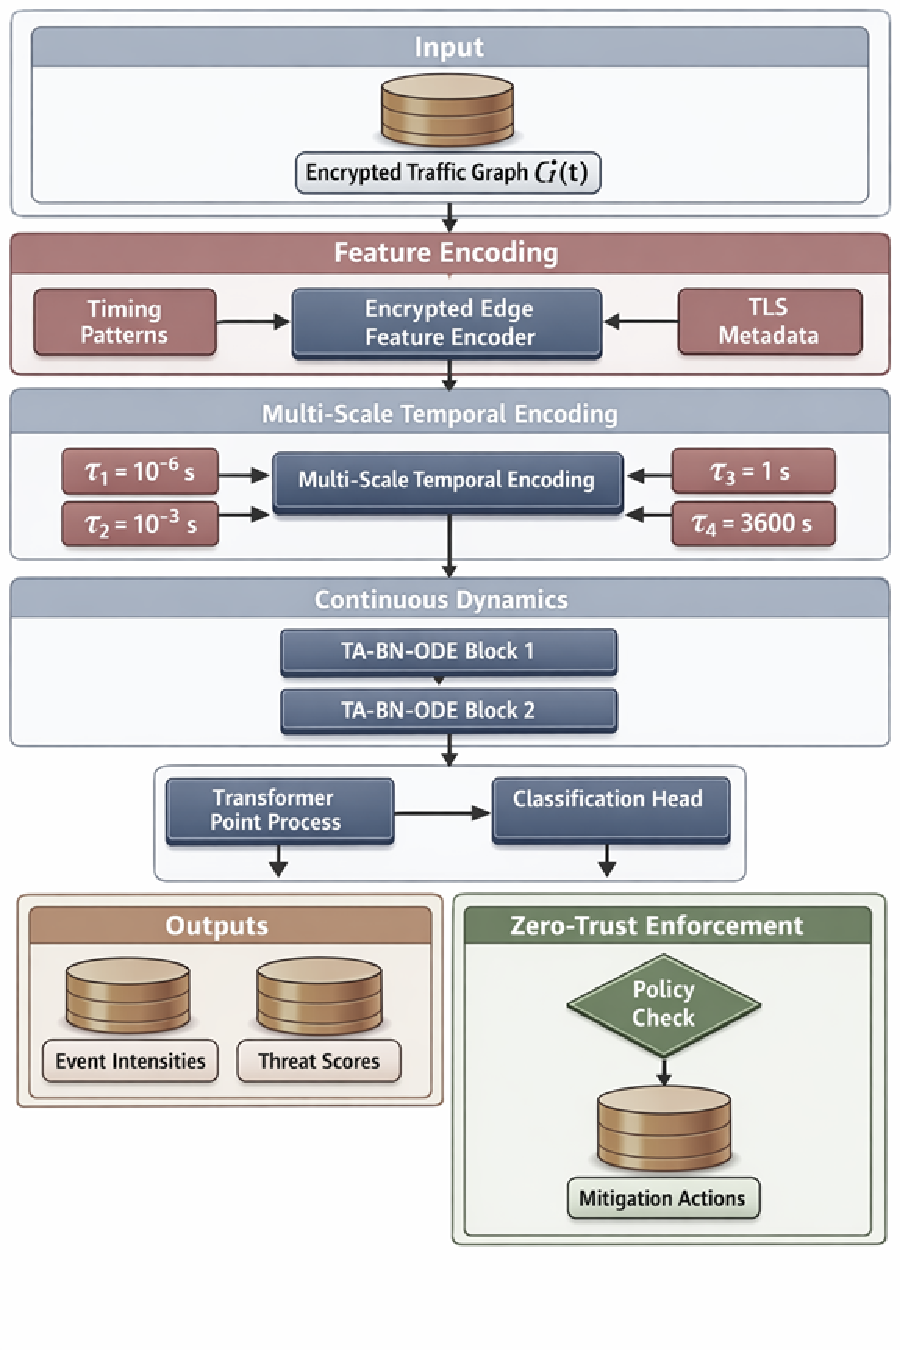
\includegraphics[width=0.70\textwidth]{figures/fig_CT-TGNN_architecture.pdf}
\vspace{-0.5cm}
\caption{CT-TGNN architecture: continuous-time graph dynamics
as a learnable component of Hybrid~IDPS}
\label{fig:CT-TGNN}
\end{figure}

The stochastic extension SDE-TGNN replaces the deterministic
dynamics with It\^{o} stochastic differential equations and
analytically propagates the mean and covariance via the
Fokker--Planck equation, yielding a certified radius through
classifier smoothing (Figure~\ref{fig:SDE_TGNN}). Achieved:
F1~99.0\%, ECE~0.042, certified adversarial robustness 76.2\%
at $R{=}0.25$, and cross-domain transfer of 90.5\% F1.

\begin{figure}[H]
\centering
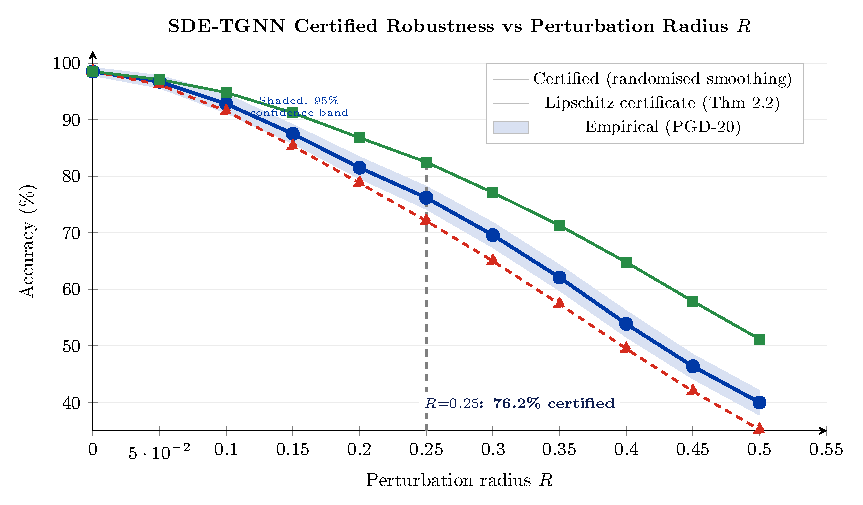
\includegraphics[width=0.80\textwidth]{figures/fig_sde_tgnn_robustness_vs_radius.pdf}
\vspace{-0.3cm}
\caption{SDE-TGNN: certified accuracy as a function of
perturbation radius}
\label{fig:SDE_TGNN}
\end{figure}

\textit{Model M2: FedLLM-API --- federated optimisation of
Hybrid~IDPS with privacy.} Coordinate-wise aggregation with
calibrated Gaussian noise and Wasserstein-distance
distributional alignment:
\begin{equation}
\theta_{t+1}=\text{TrimMean}\!\left(\{\theta_i^t\}_{i=1}^{N}\right)
+\mathcal{N}(0,\sigma^2 I),\quad
W_2(\mu_i,\mu_j)=\!\!\inf_{\pi\in\Pi(\mu_i,\mu_j)}\!\!
\sqrt{\int\!\!\|x-y\|^2 d\pi}.
\end{equation}

\textbf{Theorem~3 (Convergence under corruption).} The
algorithm converges at rate $\mathcal{O}(1/\sqrt{T})$ even
under 30\% corrupted participants while preserving
$(\varepsilon{=}0.85,\,\delta{=}10^{-5})$-differential privacy.

\begin{figure}[H]
\centering
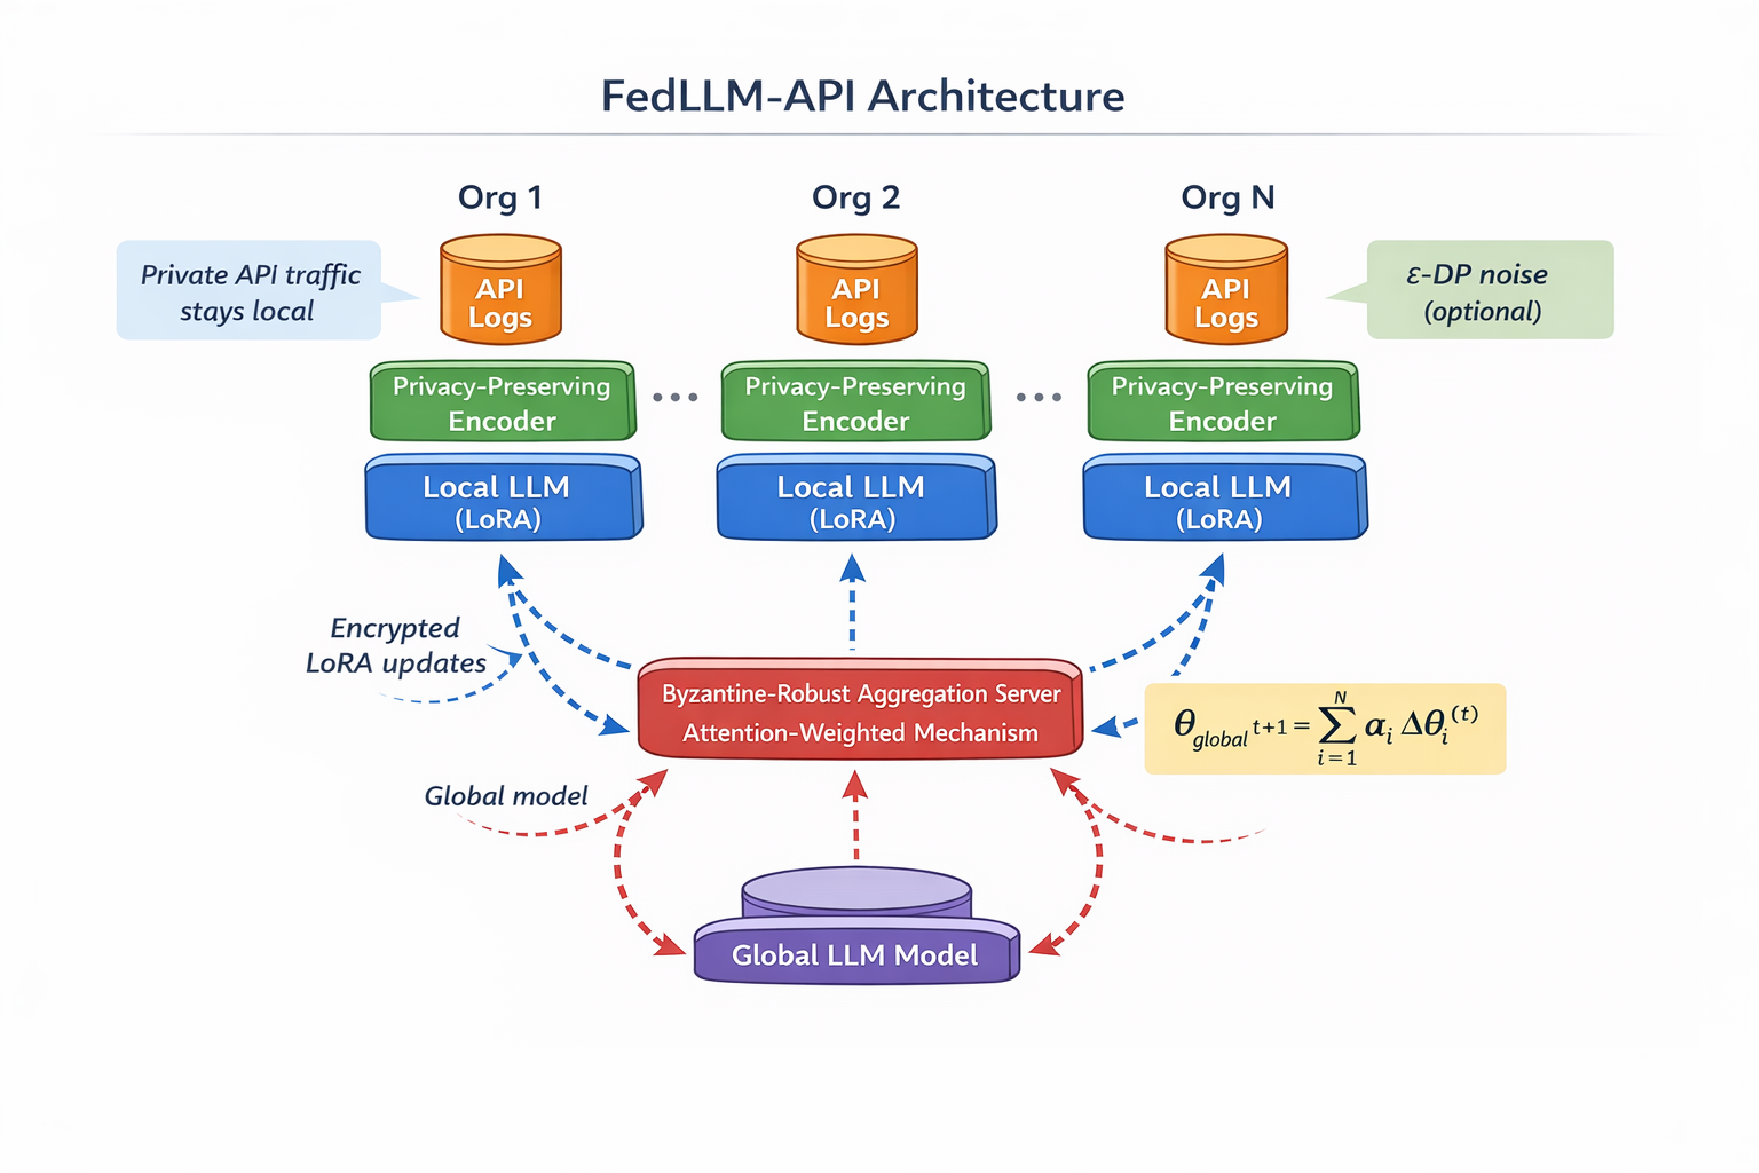
\includegraphics[width=0.80\textwidth]{figures/fig_fedllm_api_architecture.pdf}
\vspace{-0.3cm}
\caption{FedLLM-API architecture: Byzantine-resilient federated
optimisation of Hybrid~IDPS with differential privacy}
\label{fig:FedLLM}
\end{figure}

LLM integration yields 87.6\% F1 on zero-shot detection of
novel anomalous categories; at 40\% Byzantine participants the
system achieves 87.1\% accuracy versus 61.4\% for FedAvg.

\textit{Model M3: TripleE-TGNN --- multi-level temporal graph
embeddings.} Dual temporal--spatial attention and elastic
weight consolidation:
\begin{equation}
\alpha_{uv}^{(t)}=\frac{\exp(e_{uv}^{(t)})}{\sum_{w}\exp(e_{vw}^{(t)})},\qquad
\mathcal{L}_{\text{EWC}}=\mathcal{L}_{\text{task}}
+\frac{\lambda}{2}\sum_i F_i(\theta_i-\theta_i^*)^2.
\end{equation}

\begin{figure}[H]
\centering
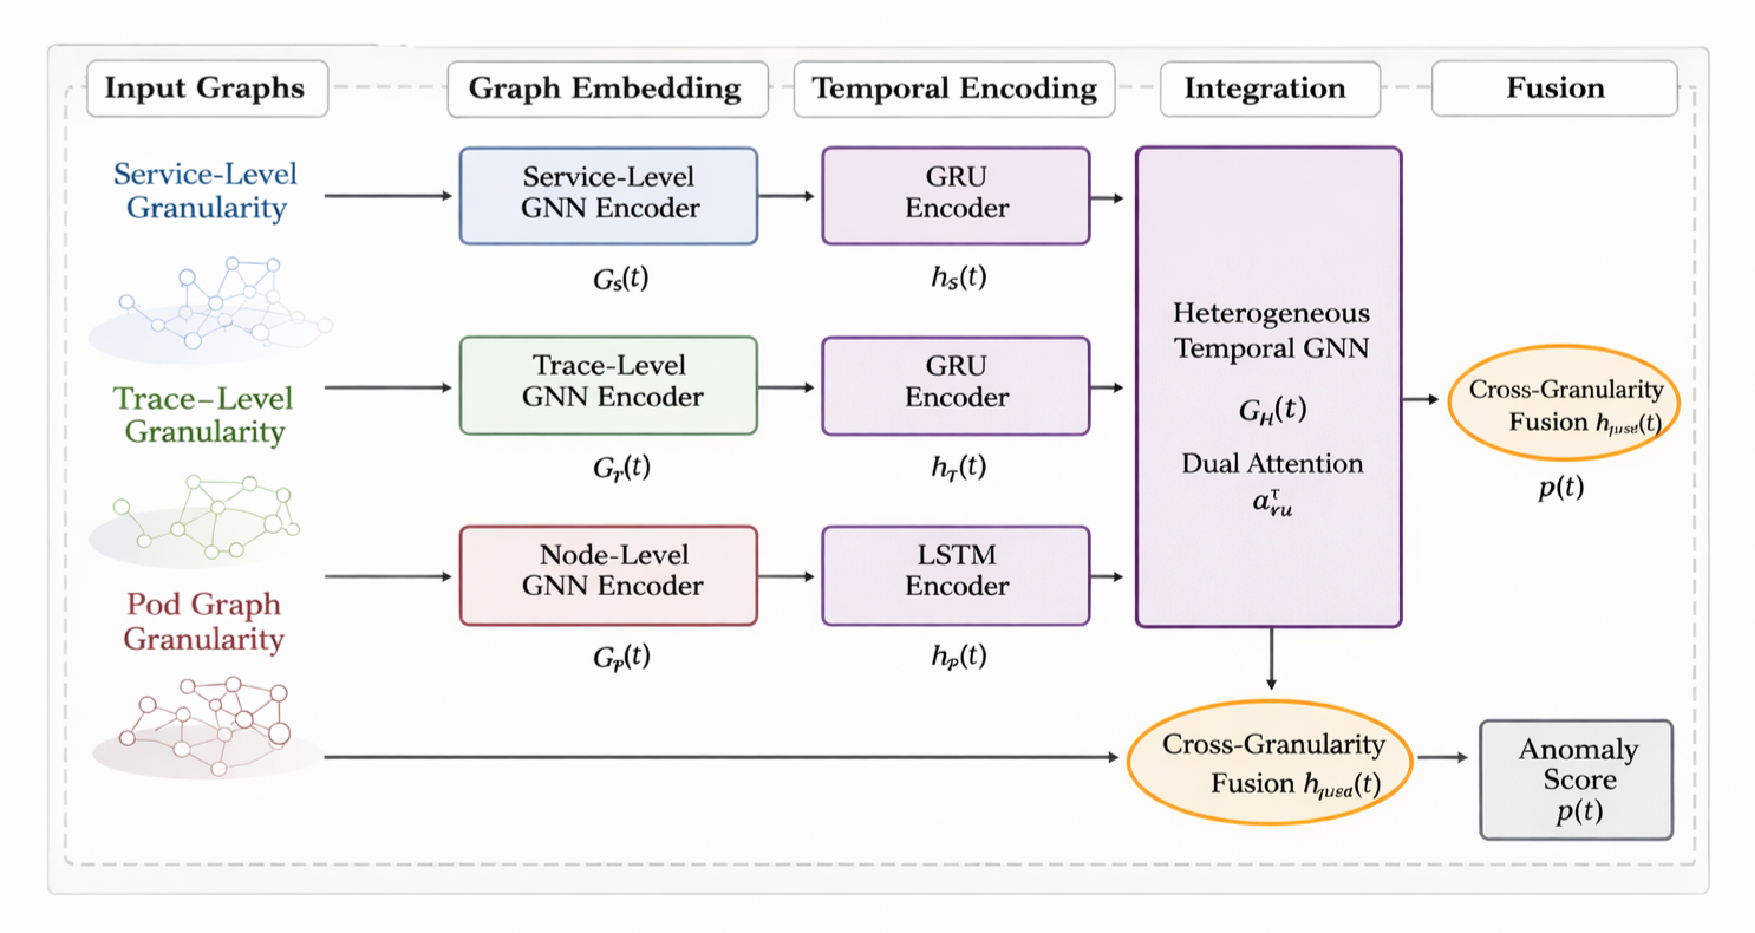
\includegraphics[width=0.95\textwidth]{figures/fig_triplee_tgnn_architecture.pdf}
\vspace{-0.4cm}
\caption{TripleE-TGNN architecture: service-, trace-, and
node-level representations with elastic weight consolidation}
\label{fig:TripleE_TGNN}
\end{figure}

Achieved accuracy of 96.8\% and 40\% reduction in computational
cost via structured sparsity.

\textit{Model M4: MambaShield --- selective state-space model
with poisoning defence.} The discrete state-space formulation
and FFT convolutions:
\begin{equation}
h_{t+1}=\bar{A}h_t+\bar{B}x_t,\quad
y_t=Ch_t+Dx_t,\qquad
\mathcal{L}_{\text{distill}}=\text{KL}\!\left(p_{\text{st}}
\Big\|\frac{1}{K}\sum_k p_{\text{tch}_k}\right).
\end{equation}

\textbf{Theorem~4 (PAC-Bayesian generalisation).}
\begin{equation}
R(\theta)\le\hat{R}(\theta)
+\sqrt{\frac{\text{KL}(\rho\|\pi)+\ln(2N/\delta)}{2N}}.
\end{equation}

\begin{figure}[H]
\centering
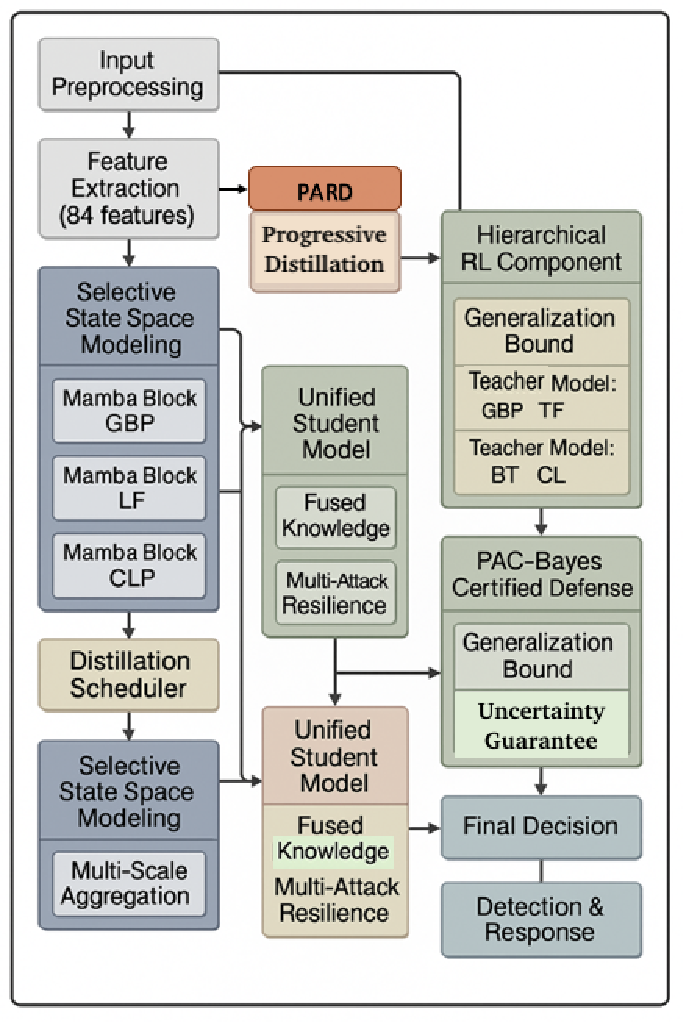
\includegraphics[width=0.65\textwidth]{figures/fig_mambashield_architecture.pdf}
\vspace{-0.3cm}
\caption{MambaShield architecture: $\mathcal{O}(L\log L)$ FFT
convolutions with progressive adversarial robustness
distillation}
\label{fig:mambashield}
\end{figure}

Under 25\% poisoning, the model achieves 91.4\% accuracy versus
73.8\% for the undefended model; inference latency 0.5~ms per
flow.

\textit{Models M5/M6: Stochastic Transformer and UC-HGP ---
uncertainty-calibrated inference.} Variational Bayesian
attention and a hierarchical Gaussian process:
\begin{equation}
q_\phi(\alpha)=\mathcal{N}(\mu_\phi,\sigma_\phi^2),\qquad
\mathcal{L}=\mathbb{E}_{q_\phi}[\log p(y|x,\alpha)]
-\text{KL}(q_\phi\|p),\qquad
f(x)\sim\mathcal{GP}(m(x),k(x,x')).
\end{equation}

\begin{figure}[H]
\centering
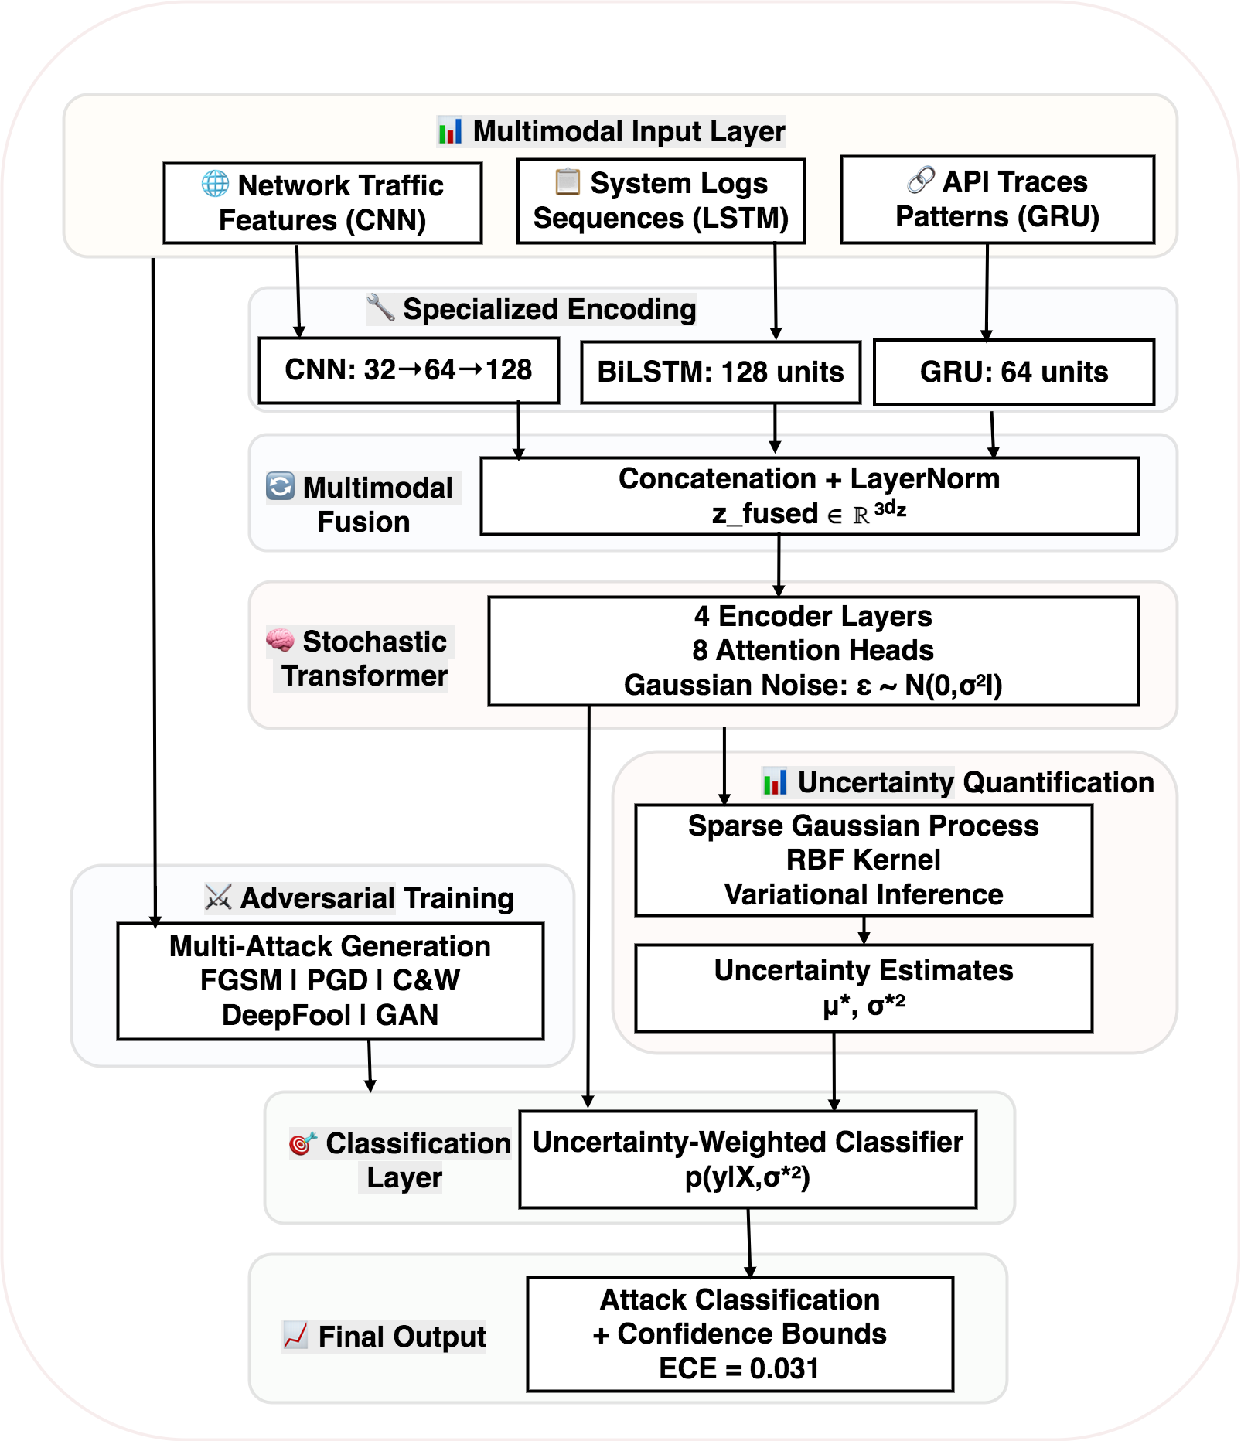
\includegraphics[width=0.80\textwidth]{figures/fig_stochastic_transformer_architecture.pdf}
\vspace{-0.3cm}
\caption{Stochastic Transformer/UC-HGP architecture:
epistemic--aleatoric uncertainty decomposition and analyst
triage}
\label{fig:UCHGP}
\end{figure}

ECE 0.078, cross-domain transfer 94.2\%, analyst-workload
reduction 43\%.

\textit{Model M7: FedGTD --- game-theoretic certification of
Hybrid~IDPS.} Stackelberg equilibrium with multiplicative
weights:
\begin{equation}
w_i^{(t+1)}=w_i^{(t)}\exp(-\eta\ell_i^{(t)}).
\end{equation}

\textbf{Theorem~5 (No regret).} Cumulative regret is bounded
by $R(T)\le 2\sqrt{T\log|\mathcal{C}|}$.

\begin{figure}[H]
\centering
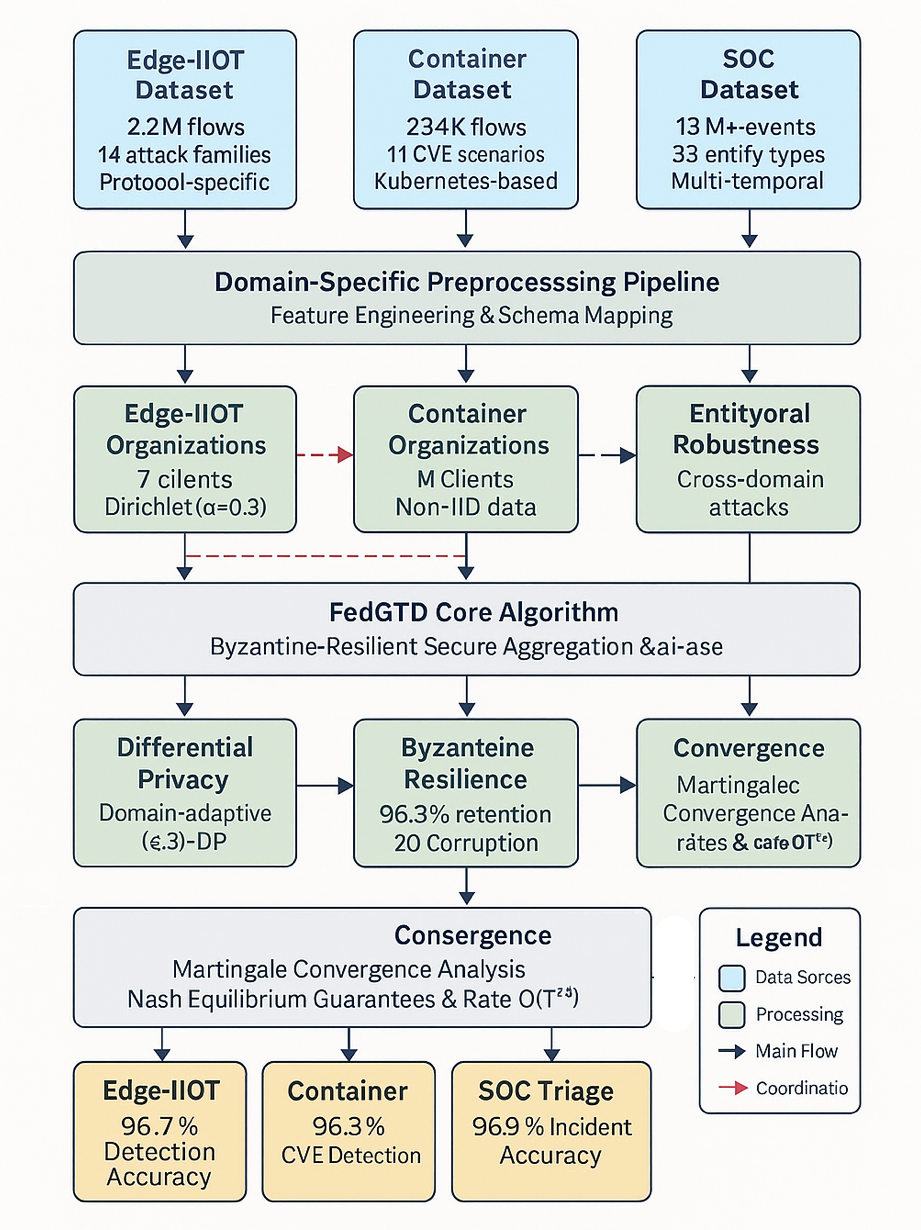
\includegraphics[width=0.80\textwidth]{figures/fig_game_theoretical_architecture.pdf}
\vspace{-0.3cm}
\caption{FedGTD architecture: game-theoretic certification
with consistency regularisation for the M1--M7 family}
\label{fig:FedGTD}
\end{figure}

Consistency regularisation couples all seven models with a
proven convergence rate and delivers 94.7\% accuracy against
adaptive adversaries versus 87.6\% for non-strategic
approaches.

\textit{CyberSecLLM foundation model.} ODE-augmented selective
state-space blocks deliver 89.1\% average zero-shot accuracy
on the CyberSecBench-11 evaluation (a 20.5-point improvement
over GPT-4) while processing million-token graph event
sequences in 2.3~seconds.

\textbf{Chapter~3} instantiates the unified mathematical
description of Hybrid~IDPS in the network-traffic protection
sector (NIDPS). Network traffic is modelled as a temporal
graph $G_t=(\mathcal{V}_t,\mathcal{E}_t,X_t)$, where nodes are
IP addresses, hosts, and services, directed edges are
communication flows, and the node feature matrix
$X_t\in\mathbb{R}^{n_t\times d}$ encodes 83~engineered features
across five categories. A unified taxonomy of 34 attack classes,
a formal PCAP/CSV-to-graph transformation pipeline, and
domain-specific hyperparameter configurations together provide
a consistent instantiation of M1--M7.

\textbf{Chapter~4} presents comprehensive experimental
validation. The evaluation spans six benchmark datasets
organised into two complementary groups, totalling 84.2~million
labelled samples and 84~attack categories (table below).

\begin{table}[H]
\centering
\caption{Benchmark datasets used in experimental evaluation}
\vspace{0.1cm}
\scriptsize
\begin{tabular}{@{}lccrcc@{}}
\toprule
\textbf{Dataset} & \textbf{Domain} & \textbf{Year} & \textbf{Records} & \textbf{Attacks} & \textbf{Feat.} \\
\midrule
\multicolumn{6}{@{}l}{\textit{Group~1: General Network Traffic (IIS3D)}} \\[2pt]
CIC-IoT-2023 & IoT & 2023 & 46.6M & 33 & 46 \\
CSE-CICIDS2018 & Enterprise & 2018 & 16.2M & 7 & 79 \\
UNSW-NB15 & Hybrid & 2015 & 2.5M & 9 & 49 \\
\midrule
\multicolumn{6}{@{}l}{\textit{Group~2: Cloud, Microservices \& Edge (ICS3D)}} \\[2pt]
Microsoft GUIDE & Cloud & 2023 & 13.7M & 15 & 51 \\
Container Security & Microservices & 2023 & 3.2M & 8 & 93 \\
Edge-IIoT & Industrial & 2022 & 2.0M & 12 & 69 \\
\midrule
\textbf{Total} & & & \textbf{84.2M} & \textbf{84} & \\
\bottomrule
\end{tabular}
\end{table}

A unified 23-metric framework spans six categories: detection
performance, calibration, uncertainty, adversarial robustness,
computational efficiency, and privacy.

\begin{figure}[H]
\centering
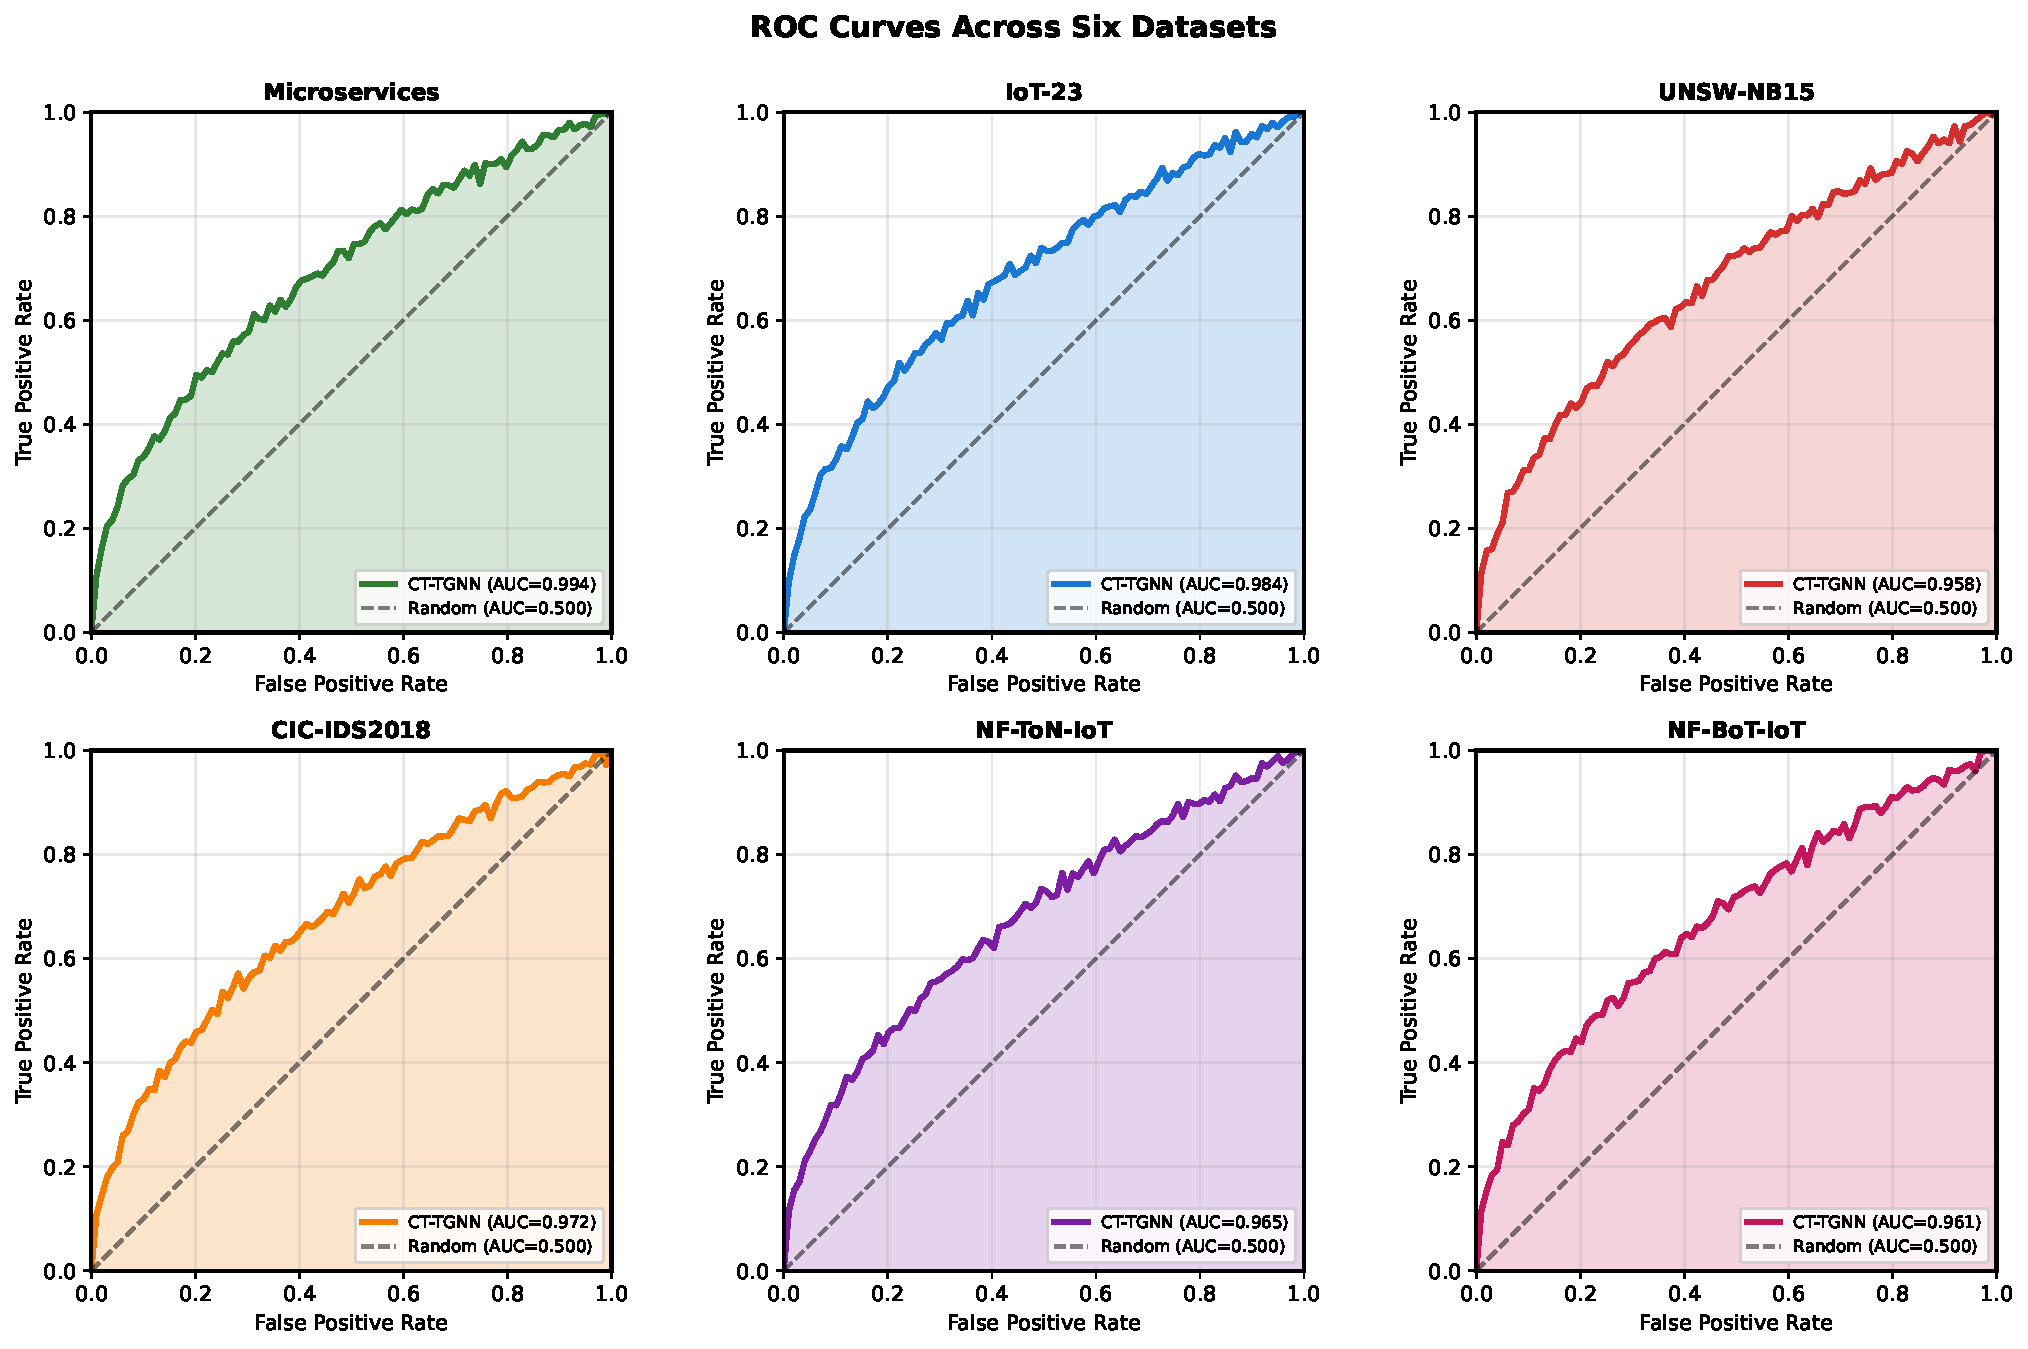
\includegraphics[width=0.96\textwidth]{figures/Figure6_ROC_Generalization.pdf}
\caption{Combined experimental evaluation of Hybrid~IDPS:
(a)~ROC curves on CIC-IoT-2023 (AUC 0.991 vs.\ 0.974);
(b)~reliability diagrams by ECE; (c)~accuracy under PGD
attacks; (d)~certified accuracy; (e)~MambaShield under
poisoning; (f)~cross-dataset accuracy heatmap}
\label{fig:roc_plot}
\end{figure}

\begin{table}[H]
\centering
\caption{Performance of the unified Hybrid~IDPS framework
across benchmark datasets}
\small
\begin{tabular}{lcccc}
\toprule
\textbf{Dataset} & \textbf{Acc.} & \textbf{F1} & \textbf{Base} & \textbf{Impr.} \\
\midrule
CIC-IoT-2023 & 94.7\% & 94.7\% & 91.8\% & +2.9 \\
CSE-CICIDS2018 & 93.9\% & 93.9\% & 89.7\% & +4.2 \\
UNSW-NB15 & 93.8\% & 93.8\% & 88.2\% & +5.6 \\
MS GUIDE & 92.1\% & 92.0\% & 87.5\% & +4.6 \\
Container Sec & 91.5\% & 91.4\% & 86.9\% & +4.6 \\
Edge-IIoT & 89.8\% & 89.7\% & 84.3\% & +5.5 \\
\bottomrule
\end{tabular}
\end{table}

\textbf{Ablation:} removing continuous dynamics --- $-6.8\%$;
multi-level embeddings --- $-8.3\%$; robust aggregation ---
$-21.4\%$; optimal transport --- $-15.8\%$; LLM component ---
$-53.4$~F1; distillation --- $-9.7\%$; variational attention
--- $-114$~ECE. \textbf{Adversarial resilience:} CT-TGNN
maintains 76.2\% at $\varepsilon{=}0.25$; the unified system
achieves 89.6\% under combined perturbations.
\textbf{Cross-domain transfer:} LibriSpeech~94.2\%~F1,
MIMIC-III/eICU~89.7\%. \textbf{Performance:} 8.7~million
events/second, 47~ms latency. \textbf{Privacy:}
$(\varepsilon{=}0.85,\,\delta{=}10^{-5})$, with accuracy
degradation of only 3.1\%. \textbf{Uncertainty:} ECE~0.078,
43\% investigation reduction. \textbf{Post-quantum
compatibility:} the Multi-Agent~PQC-IDS module delivers 96.2\%
accuracy on post-quantum protocol traffic.

\textbf{Chapter~5} integrates the developed models and
algorithms into the unified \textbf{RobustIDPS.ai} software
platform (DOI:~10.5281/zenodo.19129512), which combines
\textbf{17~neural-network models} into \textbf{10~functional
groups} (AI~Command~Center, AI~Active~Defence,
SOC~Intelligence~Suite, LLM~Attack~Surface~Testing,
MLSecOps~Standards~Compliance, AI~Security~and~Governance,
AI~Novel~Methods, AI~Data~and~Models, Multi-Agent~PQC-IDS,
System~Administration) and \textbf{51~pages} of a Progressive
Web Application. The four-layer LLM defence framework reaches
94.5\% macro-averaged detection across 517 attack scenarios
with four commercial backends (Claude, GPT-4o, Gemini,
DeepSeek). The platform deploys as a plug-in for existing
signature-based IDPS (Snort, Suricata, Zeek). User-study
validation confirms a 34\% reduction in analyst triage time.

\begin{figure}[H]
\centering
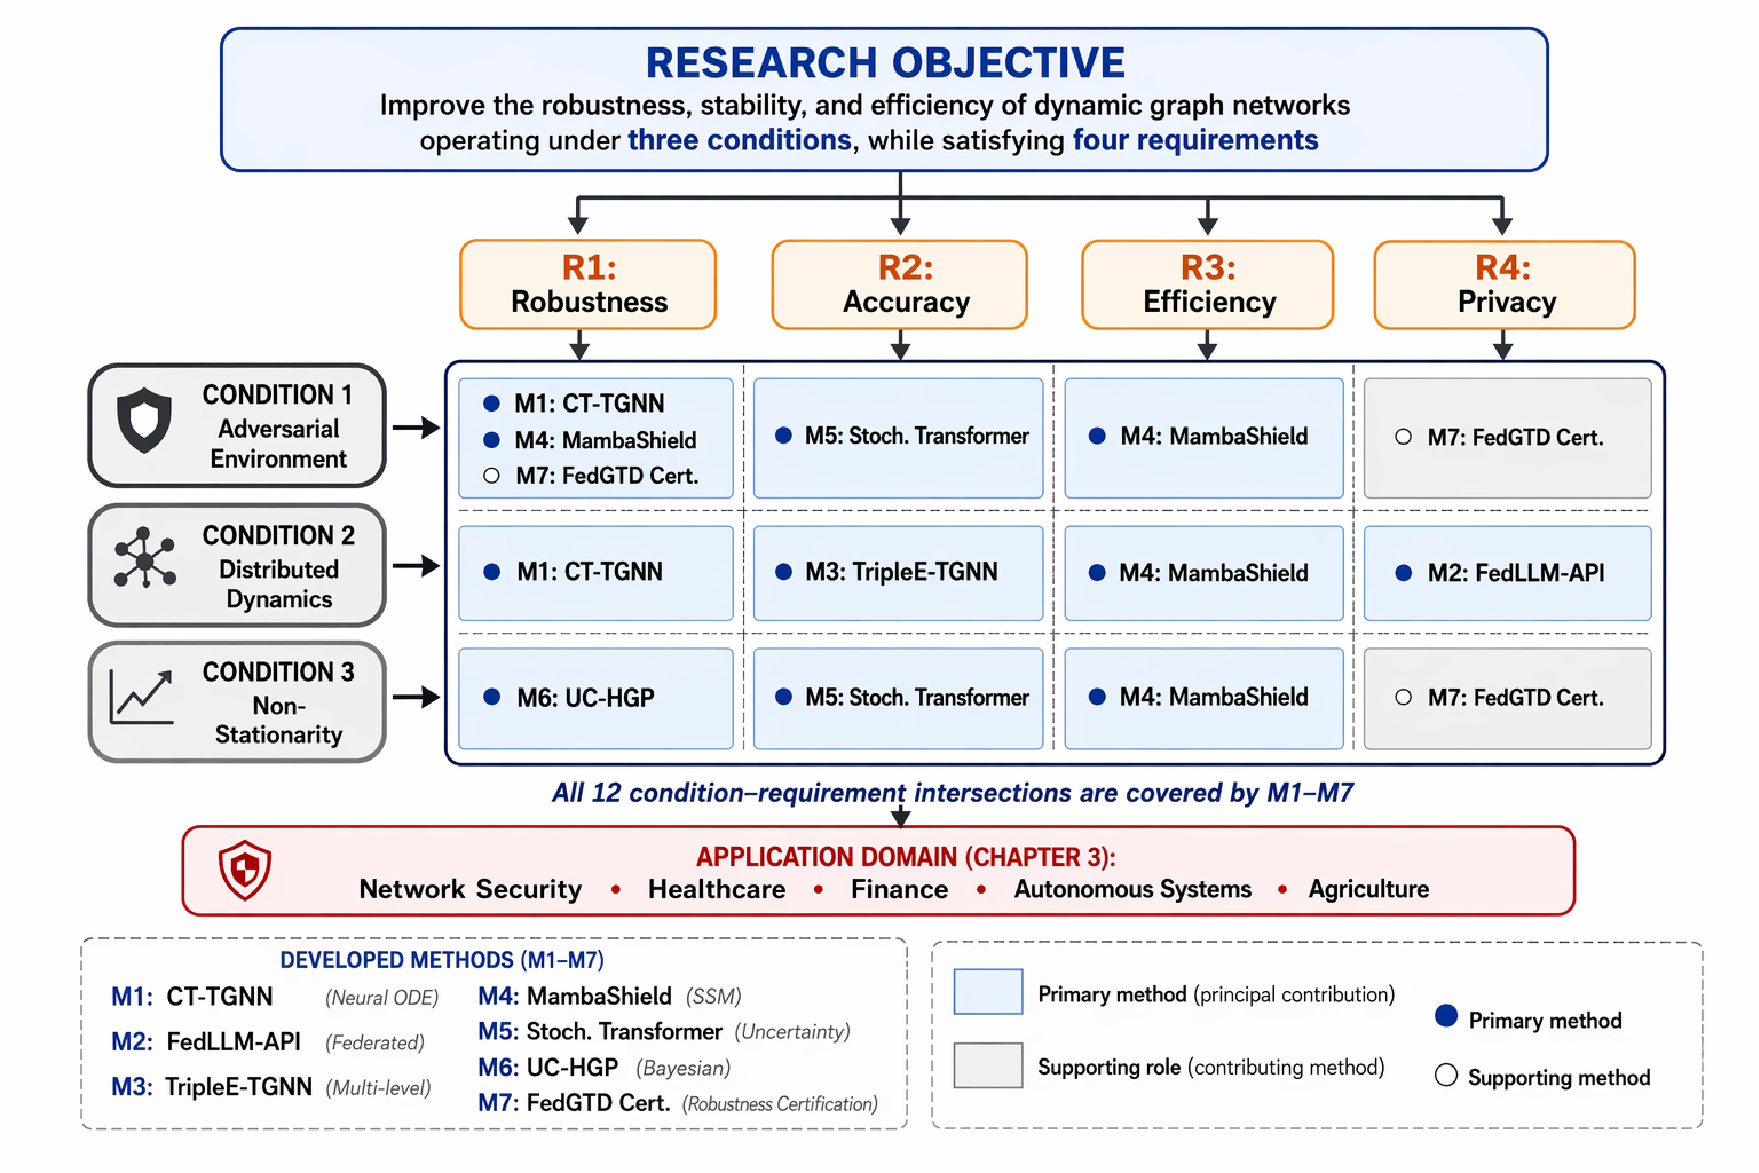
\includegraphics[width=0.96\textwidth]{figures/Main_arch_v1a.pdf}
\vspace{-0.5cm}
\caption{Architecture of the integrated RobustIDPS.ai platform
with 17~models in 10~functional groups}
\label{fig:main_arch_v1}
\end{figure}

\textbf{Chapter~6} transfers the unified Hybrid~IDPS framework
to the adjacent sector of UAV onboard-system protection with a
three-tier ``onboard~-- droneport~-- cloud'' architecture: the
onboard tier runs MambaShield inference at 0.5~ms per flow;
the droneport aggregates updates via FedLLM-API; and the cloud
tier implements game-theoretic FedGTD certification. The
transfer confirms the domain independence of the developed
mathematical and algorithmic framework.

\textbf{Implementation:}

\begin{enumerate}
\item \textit{NII~IKT~LLC} (Research Institute of Information
and Communication Technologies, Novosibirsk): integration of
poisoning-resilient network-traffic anomaly-detection models
into the operating intrusion-detection system of the
organisation, and active use of the RobustIDPS.ai software
platform by in-house cybersecurity specialists for experimental
research on information-security protocols and for continuous
network-traffic analysis \textbf{(implementation act received,
03~June 2026).}
\item \textit{Ksyrix~LLC} (Moscow): deployment of the developed
solutions within the company's network-traffic analysis and
infrastructure-protection system for detection of multi-stage
attacks and coordinated anomalies on the network-interaction
graph, uncertainty-based identification of previously unknown
anomalous patterns, and adaptation to changes in traffic
statistics \textbf{(implementation act received, 2026).}
\item \textit{Artificial Intelligence Center, NRNU~MEPhI,
Moscow:} deployment of the developed AI-based Hybrid~IDPS
framework to UAV onboard-system protection within the
three-tier ``onboard~-- droneport~-- cloud'' architecture
\textbf{(implementation act in the course of formalisation).}
\end{enumerate}

\section*{MAIN RESULTS AND CONCLUSIONS}
\addcontentsline{toc}{section}{Main Results and Conclusions}

\begin{enumerate}
\item A unified mathematical description of Hybrid~IDPS has
been formulated as the tuple
$\mathcal{H} = (\mathcal{V}_t, \mathcal{E}_t, X_t, A_t,
f_\theta, g_\psi, \pi)$ and a system of six invariant
properties P1--P6, which together form the $3\times4$
condition--requirement matrix that organises the M1--M7
family.

\item CT-TGNN and SDE-TGNN models of certified continuous-time
graph dynamics have been developed with multi-scale dynamics
and Lipschitz-based robustness certification: F1~99.0\%,
ECE~0.042, certified robustness 76.2\% at $R{=}0.25$, and
cross-domain transfer of 90.5\%.

\item The federated algorithm FedLLM-API has been created with
robust aggregation, $(\varepsilon,\delta)$-differential
privacy, and optimal-transport alignment; it converges at
$\mathcal{O}(1/\sqrt{T})$ with 40\% corrupted participants;
its LLM integration achieves 87.6\%~F1 on novel attack classes.

\item TripleE-TGNN has been developed with dual attention and
elastic weight consolidation (accuracy 96.8\%, 40\% cost
reduction); MambaShield with $\mathcal{O}(L\log L)$ complexity
achieves 91.4\% under 25\% poisoning.

\item Integration of variational Bayesian attention with
Gaussian processes has been developed for calibrated inference
of Hybrid~IDPS: ECE~0.078, with 43\% reduction in analyst
workload.

\item Game-theoretic certification FedGTD has been constructed
with Stackelberg equilibria and consistency regularisation,
unifying M1--M7 with proven convergence; accuracy of 94.7\%
against adaptive adversaries.

\item The domain-specific foundation model CyberSecLLM has been
created: 89.1\% (a 20.5-point improvement over GPT-4) with
million-token processing in 2.3~s.

\item Validation on 84.2~million samples and 84~attack
categories has been completed: the unified system reaches
94.7\% (CIC-IoT), 93.9\% (CICIDS), 93.8\% (UNSW), exceeding
baselines by 2.9--5.6~p.p.

\item The RobustIDPS.ai software platform has been implemented
(DOI:~10.5281/zenodo.19129512) with \textbf{17~models} in
\textbf{10~functional groups} and \textbf{51~pages} of the web
application, a four-layer LLM defence, and the
Multi-Agent~PQC-IDS module; it achieves 94.5\% detection
across 517 attack scenarios.

\item Domain independence of the framework has been confirmed
by transfer to the UAV onboard sector
(``onboard~-- droneport~-- cloud''), and two implementation
acts have been received: from NII~IKT~LLC (Novosibirsk;
integration of poisoning-resilient models into the operating
IDS and active use of RobustIDPS.ai by in-house cybersecurity
specialists) and from Ksyrix~LLC (Moscow; network-traffic
analysis and infrastructure protection using graph models,
uncertainty estimation, and drift adaptation); the act from
the AI Center of NRNU~MEPhI, Moscow (UAV onboard deployment),
is in the course of formalisation.
\end{enumerate}

The combined results provide a simultaneous resolution of the
adversarial-resilience, robustness, efficiency, distributed,
human-factor, and non-stationary properties of Hybrid~IDPS
through a unified mathematical description and a consistent
family of Models and algorithms M1--M7, integrating
continuous-time graph dynamics, optimal transport, Bayesian
inference, selective state-space models, and game theory.

\vspace{1cm}

\section*{PUBLICATIONS ON THE TOPIC OF THE DISSERTATION}
\addcontentsline{toc}{section}{Publications on the Topic of the Dissertation}

\sloppy

\subsection*{Articles in journals indexed in Scopus/Web of Science}

\begin{enumerate}
\item \textit{Anaedevha R.N., Trofimov A.G., Borodachev Y.V.} Uncertainty-Calibrated Hierarchical Gaussian Processes for Intrusion Detection with Multi-Scale Temporal Modeling // Neurocomputing. 2026. V.677. P.133105. DOI:~10.1016/j.neucom.2026.133105

\item \textit{Anaedevha R.N., Trofimov A.G., Borodachev Y.V.} MambaShield: Selective State-Space Models for Poisoning-Resilient Sequential Modeling // Expert Systems with Applications. 2026. P.131175. DOI:~10.1016/j.eswa.2026.131175

\item \textit{Anaedevha R.N., Trofimov A.G., Borodachev Y.V.} Temporal Adaptive Neural Ordinary Differential Equations with Deep Spatio-Temporal Point Processes for Real-Time Network Intrusion Detection // Complex and Intelligent Systems. Springer. 2026. DOI:~10.1007/s40747-026-02291-7

\item \textit{Anaedevha R.N., Trofimov A.G.} Improved Robust Adversarial Model against Evasion Attacks on Intrusion Detection Systems // Optical Memory and Neural Networks. 2024. V.33(Suppl.3). Pp.S414--S423. DOI:~10.3103/S1060992X24700681

\item \textit{Anaedevha R.N. et al.} Cyber Security Framework for Nigerian Civil Aviation Authority // International Journal of Advances in Scientific Research and Engineering. 2020. V.6(1). Pp.188--195. DOI:~10.31695/IJASRE.2020.33695
\end{enumerate}

\subsection*{Conference proceedings}

\begin{enumerate}
\setcounter{enumi}{5}
\item \textit{Anaedevha R.N., Trofimov A.G.} Integrated Deep Q-Networks and Actor-Critic Models for Enhanced Poisoning Attack Detection // 2025 Conf.\ Young Researchers in Electrical and Electronic Engineering (ElCon). IEEE Xplore. 2025.

\item \textit{Anaedevha R.N.} Application of Machine Learning Models for Device Identification in Wireless Network Traffic // 2024 ElCon. IEEE Xplore. 2024. Pp.104--110. DOI:~10.1109/ElCon61730.2024.10468413

\item \textit{Anaedevha R.N., Trofimov A.G.} Stochastic Multimodal Transformer with Uncertainty Quantification for Robust Network Intrusion Detection // Advances in Neural Computation, Machine Learning, and Cognitive Research IX. NEUROINFORMATICS 2025. Springer. DOI:~10.1007/978-3-032-07690-8\_35

\item \textit{Anaedevha R.N. et al.} Sustainable Business Model for Airline Operation in a Developing Economy // Proc.\ Intl.\ Conf.\ Science, Technology, Education, Arts, Management. 2018. Pp.167--174.

\item \textit{Anaedevha R.N., Trofimov A.G.} SDE-TGNN: Multi-Scale Temporal Graph Neural Network with Stochastic Dynamics for Cloud and Industrial Network Intrusion Detection // Proc.\ 27th IEEE Int.\ Conf.\ Young Professionals in Electron Devices and Materials (EDM-2026), Altai Republic, Russia. IEEE Xplore. 2026.
\end{enumerate}

\subsection*{Accepted for publication}

\begin{enumerate}
\setcounter{enumi}{9}
\item \textit{Anaedevha R.N., Trofimov A.G., Borodachev Y.V.} Stochastic PAC-Bayesian Transformers for Network Intrusion Detection and NLP Applications // Knowledge and Information Systems. Springer. 2025. Accepted.

\item \textit{Anaedevha R.N., Trofimov A.G., Borodachev Y.V.} Byzantine-Resilient Stochastic Games for Federated Multi-Cloud Intrusion Detection // Complex and Intelligent Systems. Springer. 2025. Accepted.
\end{enumerate}

\subsection*{Under review}

\begin{enumerate}
\setcounter{enumi}{11}
\item \textit{Anaedevha R.N., Trofimov A.G.} TripleE-TGNN: Triple-Embedding Temporal Graph Neural Networks for Multi-Granularity Microservices Security // IEEE Trans.\ Dependable and Secure Computing. 2026.

\item \textit{Anaedevha R.N., Trofimov A.G., Borodachev Y.V.} PQ-IDPS: Adversarially Robust Intrusion Detection for Post-Quantum Encrypted Traffic // IEEE Trans.\ Neural Networks and Learning Systems. 2026.

\item \textit{Anaedevha R.N., Trofimov A.G., Borodachev Y.V.} FedLLM-API: Privacy-Preserving LLM Federation for Zero-Day API Threat Detection // IEEE Trans.\ Information Forensics and Security. 2026.

\item \textit{Anaedevha R.N., Trofimov A.G., Borodachev Y.V.} CT-TGNN: Continuous-Time Temporal Graph Neural Networks for Real-Time Threat Propagation // IEEE Trans.\ Services Computing. 2026.

\item \textit{Anaedevha R.N., Trofimov A.G., Borodachev Y.V.} Hybrid Spatial-Temporal Deep Learning for Privacy-Preserving Encrypted Traffic Intrusion Detection // IEEE Access. 2026.

\item \textit{Anaedevha R.N., Trofimov A.G., Borodachev Y.V.} Differentially Private Optimal Transport for Multi-Cloud Intrusion Detection // IEEE Access. 2026.

\item \textit{Taremwa M., Anaedevha R.N., Trofimov A.G.} Robust Audio-Image Steganography using Cross-Modal Transformer Models // Journal of Computer Virology and Hacking Techniques. Springer. 2024.
\end{enumerate}

\end{document}
